\documentclass[11pt,a4paper]{article}

% Packages
\usepackage[utf8]{inputenc}
\usepackage[T1]{fontenc}
\usepackage{amsmath,amssymb,amsthm}
\usepackage{physics}
\usepackage{geometry}
\usepackage{hyperref}
\usepackage{booktabs}
\usepackage{graphicx}
\usepackage{xcolor}

\geometry{margin=1in}

\newtheorem{theorem}{Theorem}[section]
\newtheorem{lemma}[theorem]{Lemma}
\newtheorem{corollary}[theorem]{Corollary}

% === Canonical macros shared across article.tex and popular1.tex ===
\newcommand{\M}{M}              % emergent spacetime manifold
\newcommand{\Sspace}{S}         % substrate / pattern space
\newcommand{\Tsub}{T}           % substrate time parameter
\newcommand{\gmunu}{g_{\mu\nu}} % metric
\newcommand{\Tvis}{T^{\mu\nu}_{\mathrm{vis}}} % visible stress-energy
\newcommand{\TS}{T^{\mu\nu}_{S}}             % S-sector stress-energy
\newcommand{\Jsig}{J^\nu_\sigma}            % exchange current between sectors
\newcommand{\LamUV}{\Lambda_{\!*}}          % UV scale in Sint
% Gravitational coupling
\newcommand{\alphag}{\alpha}                % gravitational coupling (not fine-structure!)
% Efficiencies & sector qualities
\newcommand{\Qmat}{Q_{\mathrm{mat}}}
\newcommand{\Qgam}{Q_{\gamma}}
\newcommand{\Qtot}{Q_{\mathrm{tot}}}
\newcommand{\epsmat}{\varepsilon_{\mathrm{mat}}}
\newcommand{\epsgam}{\varepsilon_{\gamma}}
% SME-related parameters
\newcommand{\ktildee}{\tilde{\kappa}_{e-}}
\newcommand{\XiJK}{\Xi_{JK}}
% S-mediator kernel and distance
\newcommand{\Kern}{K_\sigma}
\newcommand{\Dsig}{d_\sigma}
\newcommand{\Lsig}{\lambda_\sigma}
% Selection operator
\newcommand{\Osel}{\mathcal{O}_{\!S}}  % selection operator (dim 4)

% --- Aether-resonance macros ---

% Structural kernel on S
\providecommand{\Ksig}{K_\sigma}

% Structural range lambda_sigma (sometimes written as \lsig)
\providecommand{\lsig}{\lambda_\sigma}

% Substrate power P_sigma
\providecommand{\Psig}{P_\sigma}

% Pump rate (events per second)
\providecommand{\PumpRate}{\Gamma_{\mathrm{pump}}}

% Effective temperature used in Sec. 8 (I wrote \Temp there)
\providecommand{\Temp}{T}

% fix anchors (?)
\makeatletter
\renewcommand{\theHequation}{\thesection.\arabic{equation}}
\makeatother

\title{Aether Resonance: Substrate-Local FTL Transfer in a Discrete Substrate}
\author{}
\date{}

\begin{document}

\maketitle

\begin{abstract}
We propose and analyse a speculative framework in which observable spacetime $(M,g)$ with light speed $c$ emerges from an underlying discrete substrate with global update order $(\Tsub=0,1,2,\ldots)$ and a second, \emph{structural} notion of proximity $(\Sspace,\Dsig)$ that measures algorithmic similarity of local patterns. A weak, substrate-local coupling in $(\Sspace)$ --- ``aether resonance'' --- allows energy and information to be redistributed along $\Sspace$-geodesics within a single substrate tick, appearing as superluminal (FTL) in $(M)$ while remaining causal in $(\Sspace)$. 

Starting from a total action $S_{tot}$ that couples visible fields to an $S$-mediator and a pattern-selection operator $\Osel$, we derive the field equations, conservation laws, and consistency conditions. Key results include: (i) a split conservation law for visible and $S$-sector stress-energy with exchange current $\Jsig$, (ii) an explicit proof that the Einstein equations require a \emph{universal} gravitational coupling $\alphag\equiv 1$ even in the presence of exchange, (iii) construction of a retarded $S$-mediator that realises locality and exponential falloff in $\Dsig$, (iv) an information-theoretic interpretation of resonance as a ``similarity pump'' with entropy cost, (v) an effective substrate distance $\Dsig$ and ``distance ladder'' relating microscopic pattern moves to macroscopic displacements in $(M)$, (vi) a thermodynamic resource inequality that bounds FTL bitrate by entropy production, (vii) a modified Lieb-Robinson bound with explicit conditions, (viii) a \textbf{thermodynamic resource inequality} with bitrate bounds, (ix) an \textbf{anisotropy budget}, (xi) a \textbf{proof that the gravitational coupling of the $S$-sector is fixed to $\alphag=1$ by the Bianchi identity}, and (xii) stringent, \textbf{no-loophole} experiments (E1–E3) with mapped parameter inference and multiple-test correction.
\end{abstract}

\section{Introduction and Motivation}

Relativity and quantum mechanics provide a consistent, locally causal description of all known phenomena over many orders of magnitude. At the same time, they leave open the question of whether spacetime and its light-cone structure are fundamental, or whether both might instead emerge from some deeper, discrete substrate.

Questions of this kind are also addressed in discrete and emergent approaches to quantum gravity, where spacetime is reconstructed from more primitive combinatorial structures. Examples include causal sets, causal dynamical triangulations, and quantum graphity, which start from locally finite partial orders, ensembles of triangulations, or dynamical graphs and recover continuum behaviour in a coarse-grained limit~\cite{surya2019_cst,loll2019_cdt,konopka2008_graphity}. Our goal here is not to propose yet another specific microscopic model, but to explore what happens if such a substrate also supports a second notion of proximity in a pattern space $S$ and a corresponding substrate-local coupling that can project as FTL in the emergent spacetime $M$.

In this work we investigate the speculative but internally consistent hypothesis that:

\begin{enumerate}
\item Observable spacetime $(M)$ with light speed $(c)$ arises as an effective, coarse-grained description of a discrete substrate with global update ordering $(T=0,1,2,\ldots)$.
\item There exists a second notion of distance --- \textbf{structural proximity} in a pattern space $(\Sspace,\Dsig)$ --- in which two local substrate configurations are ``close'' if they are algorithmically isomorphic.
\item A weak, substrate-local coupling in $(\Sspace)$ --- \textbf{aether resonance} --- allows energy and information to be redistributed ``in place'' in $(\Sspace)$, which is experienced as FTL in $(M)$.
\end{enumerate}

The question is whether this can be made \textbf{physically coherent}: compatible with conservation laws, with the Equivalence Principle and observed Lorentz symmetry, with quantum mechanics and Bell tests, with known high-energy and astrophysical constraints, and with existing no-go theorems on FTL signalling. We aim to show that this is possible in a tightly constrained way that yields concrete, conservative experimental results, and \textbf{falsifiable consequences}. Conventional FTL scenarios in general relativity exploit exotic spacetime geometries such as warp bubbles or traversable wormholes~\cite{alcubierre1994_warp,morris1988_wormholes}; in contrast, we keep the metric sector of GR fixed and explore a substrate-level mechanism.

Throughout this work we treat the visible sector as standard quantum
field theory on $(M,g)$, with local Hamiltonian dynamics and the usual
Born-rule interpretation.  The substrate and the $S$-mediator are
introduced at an effective level as additional degrees of freedom that
mediate a pattern-dependent channel for energy and information
transfer.  We do not attempt to quantize the substrate explicitly; for
the purposes of the modified Lieb--Robinson bound and the causality
proof it is sufficient that the combined dynamics be generated by a
Hamiltonian on a Hilbert space and that the $S$-sector obey the
retardation, sparsity, and cost assumptions spelled out in
Appendix~\ref{app:assumptions}.  The proposed experiments are therefore tests of an
\emph{extra} channel on top of standard quantum theory in the visible
sector, rather than modifications of the linear structure of quantum
mechanics itself.

\subsection{Relation to existing approaches}
\label{subsec:related-work}

Several existing frameworks introduce preferred structures, small departures from exact local Lorentz invariance, or an underlying discrete substrate from which spacetime emerges. Here we position the present proposal with respect to the most relevant lines of work and highlight what is genuinely new.

\paragraph{Discrete and emergent spacetime.}
Approaches such as causal set theory, causal dynamical triangulations (CDT), and quantum graphity start from a fundamentally discrete structure---a locally finite partial order, ensembles of triangulations, or dynamical graphs---from which continuum spacetime and locality emerge in a coarse-grained limit~\cite{surya2019_cst,loll2019_cdt,konopka2008_graphity}. These models show that discreteness can coexist with approximate Lorentz invariance and with nonlocal microscopic structure. Our framework is agnostic about the microscopic details, but shares the basic premise that the observed manifold $(M,g)$ need not be fundamental. The distinctive feature here is the introduction of a \emph{second} proximity structure $(S,d_\sigma)$, together with a weak, pattern-dependent coupling that is strictly local in $S$ yet can redistribute energy and information superluminally in $M$ while remaining compatible with a globally well-defined substrate time.

\paragraph{Cellular and quantum cellular automata substrates.}
Discrete-time dynamics with a global update ordering are familiar from cellular automata and from quantum cellular automata (QCA), which provide general frameworks for local deterministic and local unitary evolution on discrete lattices and graphs~\cite{thooft2016_ca,farrelly2020_qca}. Such models can reproduce relativistic wave equations and even full quantum field theories in appropriate continuum limits. Our postulate P1 (discrete dynamics and global ordering) is in this spirit: we assume that there \emph{exists} some CA/QCA-like substrate that gives rise to standard QFT on $(M,g)$ at low energies, but we do not attempt to specify it. Instead, we add an additional structure---the pattern space $S$, a computable metric $d_\sigma$, and a substrate-local coupling in $S$---and explore the consequences of this extra channel. In this sense aether resonance is ``QCA + an additional, structure-selective channel'', rather than a new microscopic model of the substrate itself.

\paragraph{Einstein--\ae ther and khronometric gravity.}
Einstein--\ae ther and khronometric models introduce a unit timelike vector field $u^\mu$ that picks out a preferred foliation while keeping the gravitational sector close to GR~\cite{jacobson2004_einstein_aether,jacobson2008_einstein_aether_status,horava2009_qg_lifshitz,blas2011_horava_models}. These theories propagate additional modes and are tightly constrained by post-Newtonian tests, binary pulsars, and by the near-equality of the speed of gravity and the speed of light inferred from GW170817 and GRB 170817A~\cite{yagi2014_einstein_aether_pulsars,oost2018_einstein_aether_gw170817,baker2017_gw170817_mg,creminelli2017_dark_energy_gw170817,will2014_confrontation_gr}. Our $L_S$ in Eqs.~(3.1A)–(3.1C) is chosen from this well-studied class, but we adopt a \emph{constraint-only, minimal khronon} regime: the unit timelike vector is enforced by a Lagrange multiplier, we set $c_T=c$, and we do not allow new propagating metric degrees of freedom. As a result, the strong constraints on modified gravity are automatically respected. The preferred structure that is phenomenologically relevant in our framework lives primarily in the pattern space $S$ and in the selection operator $O_S$, which together generate an additional channel for energy/information transfer rather than a simple modification of dispersion relations.

\paragraph{Standard-Model Extension and Lorentz-violation searches.}
The Standard-Model Extension (SME) provides a systematic parametrization of small Lorentz-violating coefficients in photon and matter sectors~\cite{kostelecky2002_photon_sme,kostelecky2009_photon_nonminimal}. Modern resonant-cavity and clock-comparison experiments constrain these coefficients at the level of $\Delta\nu/\nu \sim 10^{-18}$ and below~\cite{eisele2009_light_isotropy,nagel2015_lorentz10minus18,kostelecky2018_clock_tests}. Sections~11 and Appendix~\ref{app:sme-coupling} explicitly borrow the SME language: we define an ``anisotropy budget'' and translate aether-resonance effects into effective photon-sector coefficients $\tilde{\kappa}^{e-}_{JK}$. In contrast to a generic SME analysis, however, these coefficients are not free parameters: in our model they are tied to a specific mechanism (substrate locality in $S$ combined with $O_S$ and the kernel $K_\sigma$), and to concrete experiments (E1–E3) with pre-specified parameter maps. Null results in those experiments therefore become bounds on tightly constrained combinations of SME coefficients rather than isolated numbers.

\paragraph{Locality bounds, Bell nonlocality, and fast-light analogues.}
In standard local quantum lattice systems, the Lieb–Robinson bound quantifies an emergent light cone for the propagation of operator commutators~\cite{lieb1972_lr}. For systems with long-range interactions this is generalized to ``soft'' or distorted light cones whose shape depends on the interaction tail~\cite{fossfeig2015_longrange_lr,tran2020_hierarchy_lightcones}. In quantum information, Bell nonlocality and related no-signalling theorems show how nonlocal correlations can coexist with relativistic causality~\cite{brunner2014_bell_nonlocality}, while fast-light experiments demonstrate that superluminal group velocities do not imply superluminal information transfer~\cite{stenner2003_fast_light}. Our modified Lieb–Robinson bound (Sec.~9) and the categorical causality proof (Sec.~10) are best viewed as substrate-level analogues of these results: individual influence steps can be superluminal in the emergent spacetime $M$, but every allowed influence chain is monotone in the substrate time $\tau$, and the effective commutators outside the usual light cone are exponentially suppressed in $d_\sigma$ and retarded at finite mediator speed $c_S$.

\paragraph{Thermodynamics of information and pattern-space methods.}
The thermodynamic resource inequality in Sec.~8 rests on Landauer's principle---the $k_B T \ln 2$ cost of reliably erasing a bit---and on its experimental confirmations in single-bit systems~\cite{landauer1961_irreversibility,berut2012_landauer_exp,jun2014_landauer_precision}. We do not propose any violation of this principle; instead, we derive a bound that says that any sustained FTL bitrate through the $S$-channel must pay a conventional Landauer cost multiplied by an efficiency factor involving the pattern quality factor $Q$ and the similarity kernel $K_\sigma$. The operational pattern metric $d_\sigma$ is in turn built from gauge- and diffeomorphism-invariant features, including topological signatures (persistent homology) and dynamical response features that can be extracted using techniques from topological data analysis and physical reservoir computing~\cite{carlsson2009_topology_data,tanaka2019_physical_reservoir,vandersande2017_photonic_reservoir}. In this way the abstract notion of ``algorithmic similarity'' is connected to concrete, calibration-ready tools.

\paragraph{Conventional FTL geometries in general relativity.}
There is a long-standing literature on effective FTL travel within GR based on exotic spacetime geometries such as Alcubierre's warp drive and traversable wormholes~\cite{alcubierre1994_warp,morris1988_wormholes}. These scenarios keep local microphysics unchanged but rely on large curvature and violations or saturation of energy conditions. By contrast, the present proposal keeps GR unchanged in the metric sector and instead introduces a new, pattern-selective channel that is local in $S$ and nonlocal in $M$. From the point of view of observational tests, this means that our framework should be constrained alongside SME coefficients and long-baseline Lorentz tests, rather than through the viability of exotic stress–energy tensors.

\section{Postulates and Formalisms}

(\textbf{Notation hint:} For unified symbols, units, and macros, see Appendix~\ref{app:nomenclature}.)

\subsection{P1. Discrete Dynamics and Global Ordering}

The substrate evolves in discrete steps $(T)$. All causality is \textbf{monotonic in $(T)$}.

\subsection{P2. Two Proximities and a Projection}

\begin{itemize}
\item \textbf{$(M)$}: emergent spacetime with metric $(g_{\mu\nu})$, where ordinary matter moves locally and obeys relativity.
\item \textbf{$(S)$: The Pattern Bundle.} We define the total pattern space as a bundle $\tilde{S}$ over the emergent spacetime $M$. For each point $x \in M$, the fiber $S_x$ consists of the equivalence classes of microscopic substrate states supported in a neighborhood of $x$. The total space is $\tilde{S} = \bigsqcup_{x \in M} S_x$.
\item \textbf{$(\pi)$: The Projection.} The map $\pi: \tilde{S} \to M$ is the canonical bundle projection, mapping any pattern $\sigma_x \in S_x$ back to its spacetime location $x$.
\item \textbf{$(d_\sigma)$: Structural Metric.} The distance $d_\sigma$ is defined \textbf{on the fibers}: it measures the algorithmic or structural similarity between two patterns $\sigma \in S_x$ and $\sigma' \in S_{x'}$, independent of their base points $x$ and $x'$.
\end{itemize}

A schematic of the bundle structure is shown in Fig.~\ref{fig:bundle}.

\begin{figure}[t]
\centering
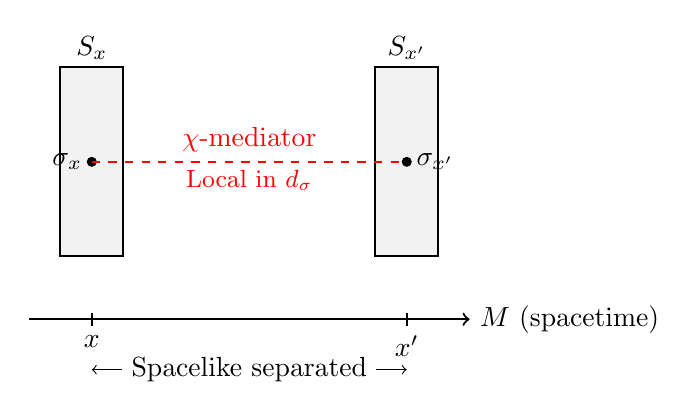
\begin{tikzpicture}[scale=0.8]
  % Base manifold M
  \draw[thick, ->] (-1,0) -- (6,0) node[right] {$M$ (spacetime)};
  \draw[thick] (0,0.1) -- (0,-0.1) node[below] {$x$};
  \draw[thick] (5,0.1) -- (5,-0.1) node[below] {$x'$};
  
  % Fibers S_x
  \draw[thick, fill=gray!10] (-0.5, 1) rectangle (0.5, 4);
  \node at (0, 4.3) {$S_x$};
  \draw[thick, fill=gray!10] (4.5, 1) rectangle (5.5, 4);
  \node at (5, 4.3) {$S_{x'}$};
  
  % Patterns
  \filldraw (0, 2.5) circle (2pt) node[left] {$\sigma_x$};
  \filldraw (5, 2.5) circle (2pt) node[right] {$\sigma_{x'}$};
  
  % Connection in S
  \draw[red, thick, dashed] (0, 2.5) -- (5, 2.5) node[midway, above] {$\chi$-mediator};
  \node[red, font=\small] at (2.5, 2.2) {Local in $d_\sigma$};
  
  % Spacetime separation
  \draw[<->] (0, -0.8) -- (5, -0.8) node[midway, fill=white] {Spacelike separated};
\end{tikzpicture}
\caption{Schematic illustration of the pattern bundle $\tilde S$. Interaction is local in the pattern space fiber (dashed red line) connecting $\sigma_x$ and $\sigma_{x'}$, even though the base points $x, x'$ are spacelike separated in $M$. From the viewpoint of $M$ this appears as superluminal transfer, although every microscopic step is retarded in $\tau$.}
\label{fig:bundle}
\end{figure}

\subsection{P3. Aether Resonance – Substrate-Locality in $(S)$}

There exists a coupling that, within one tick, allows energy or information to move from one region in $M$ to another via a path in $S$ whose cost depends only on $\Dsig(s,s')$, independent of $|\pi(s) - \pi(s')|$ in $(M)$.

\subsection{P4. Conservation Laws in $(M\times S)$}

Total energy/information is conserved over the combined dynamics in $(M\times S)$, even though local budgets in $(M)$ may vary via flows in $(S)$.

\subsection{P5. Substrate classes compatible with our assumptions}
\label{subsec:substrate-classes}

Appendix~\ref{app:assumptions} collects the structural assumptions (A1)--(A9) used in the
derivation of the modified Lieb--Robinson bound, the categorical
causality proof, and the phenomenological estimates.  Here we sketch
what kinds of discrete substrates actually satisfy these assumptions.

\paragraph{Global ordering and strict retardation (A1).}
A1 is satisfied by any discrete--time dynamics in which the microscopic
update rule takes the form
\[
(s,T) \mapsto (s',T+1)
\]
with no backward steps in $T$, and in which the mediator kernel
$G_{\rm ret}$ in $S$ vanishes for $T'<T$.  Concrete examples include
cellular automata on fixed graphs with synchronous updates, and
asynchronous update schemes in which all allowed local moves advance a
global integer ``tick'' $T$ by~1.  In both cases the coarse--grained
substrate time $\tau$ can be taken as a smoothed version of~$T$.
Concrete realizations of such dynamics have been extensively studied in the literature on cellular automata and quantum cellular automata, which provide general frameworks for discrete-time local evolution and for emergent relativistic behaviour~\cite{thooft2016_ca,farrelly2020_qca}. We remain agnostic about the detailed update rule and only assume that it satisfies the structural conditions (A1)–(A9).

\paragraph{Sparsity and weak coupling (A3).}
A3 requires that each node in the substrate pattern graph participates
in at most $g<\infty$ active $S$--edges and that the corresponding
Hamiltonian perturbations $h_e$ obey $\|h_e\|\le\eta$ with
$\mu>\ln g$, where $\mu$ is the decay rate of the kernel in $S$.  This
is naturally satisfied by substrates built from:
\begin{itemize}
  \item locally finite graphs (e.g.\ nearest--neighbour lattices,
        bounded--degree random graphs, sparse small--world networks);
  \item update rules in which only a small fraction of potential edges
        are simultaneously active (e.g.\ stochastic activation with
        fixed mean degree).
\end{itemize}
In such substrates the path sums that enter the function
$\Phi(g,\eta t/\hbar)$ in Eq.~(9.2) converge and the $S$--tail cannot
become distance--independent.

\paragraph{Structure of $O_S$ and degeneracy dilution (A4).}
A4 requires that $O_S$ be constructed from higher--dimension seed
operators with $\Delta>4$, normalized so that $[O_S]=4$, and that
$\langle O_S\rangle$ vanish (or be extremely small) in homogeneous,
periodic, or thermal states because of degeneracy dilution.
Qualitatively, if there are $N\gg 1$ macroscopically equivalent ways to
embed a given mesoscopic pattern into a homogeneous background, then a
generic superposition of those embeddings yields an overlap that
scales as $1/\sqrt{N}$ or smaller.  This drives the effective quality
factor $Q$ to zero in the thermodynamic limit.  Appendix~\ref{app:degeneracy-toy-model} gives an
explicit toy model illustrating this scaling on a finite lattice.

Conversely, in carefully engineered mesoscopic platforms (Sec.~5.3)
the pattern selected by $O_S$ can be realized in only a few locations
with aligned phases, so that $Q$ can approach order unity.  This
difference between ``generic'' and ``engineered'' states is what
suppresses collider and everyday signatures while allowing sharply
tuned experiments to be sensitive.

\paragraph{Kernel structure and minimal Lorentz breaking (A5--A6).}
A5 and A6 are satisfied by substrates in which:
\begin{itemize}
  \item the similarity kernel $K_\sigma(\sigma,\sigma')$ depends only
        on a bona fide metric $d_\sigma(\sigma,\sigma')$ as in
        Eq.~(7.1), with $K_\sigma=\exp[-d_\sigma/\lambda_\sigma]$;
  \item the $u^\mu$ aether/khronon sector lies within the
        Einstein--\ae{}ther / khronometric parameter region where
        $c_T=c$ and preferred--frame effects in gravity obey existing
        bounds [cf.\ Eq.~(3.1C)].
\end{itemize}
In other words, the substrate can carry a preferred frame and an
$S$--metric without spoiling standard tests of GR provided the
aether/khronon sector is chosen conservatively.

\paragraph{Cost monotonicity and pump budget (A2, A8, A9).}
A2, A8, and A9 formalize the idea that resonance steps carry a positive
thermodynamic cost and that the pump budget is finite.  These
assumptions are satisfied whenever:
\begin{itemize}
  \item each microscopic update that changes the $S$--state dissipates
        at least $k_B\Theta\ln 2$ of entropy per bit of information, in the
        spirit of Landauer's principle;
  \item the total pump power $P_{\rm pump}$ is bounded on the relevant
        time scales.
\end{itemize}
Under these conditions we can define a cost functor $\tilde K$ as in
Appendix~D and a pump-rate $\Gamma_{\rm pump}$ as in Sec.~6.2, and the
resource inequality (8.3) follows.

These examples are not meant as a unique substrate proposal; they are
intended to demonstrate that the abstract assumptions (A1)--(A9) are
satisfied by broad classes of discrete systems rather than by a single
fine--tuned construction.

Postulates P1--P4 define the effective framework at the level of spacetime $M$, the substrate time function $\tau$, and the pattern space $S$. For some of our more technical results, in particular the modified Lieb--Robinson bound and the causality statements, we will also use a set of structural assumptions (A1--A9) collected in Appendix~\ref{app:assumptions}. These assumptions constrain the allowed substrates more strongly (for example by requiring sparsity and bounded degree of $S$-links), but they are not needed for the definition of the action or the basic split conservation laws in Sec.~\ref{sec:action}. In later sections we will be explicit about which derivations use only P1--P4 together with (A1)--(A9) and therefore apply to any substrate in this class, and which rely on additional modelling choices introduced below.

\section{Action and Field Content}

\subsection{Variational Principle}

We derive the framework from a \textbf{total action}:

\begin{equation}
\begin{split}
S_{tot} = \int d^4x \, \sqrt{-g} \left[ \frac{1}{16\pi G} R
+ \mathcal{L}_{vis}[\phi, g] + \mathcal{L}_S[\tau, u^\mu, g] \right] \\
 + \varepsilon \int d^4x \sqrt{-g}\!\int\! d\mu(\sigma)\,d\mu(\sigma')\,
\frac{O_S(x,\sigma)\,\Kern(\sigma,\sigma')\,O_S(x,\sigma')}{\LamUV^{4}},
\end{split}
\tag{3.1}
\end{equation}

where:

\begin{itemize}
\item $\mathcal{L}_{vis}$ collects all visible matter and gauge fields.
\item $\mathcal{L}_S$ is a minimal aether/khronon sector that allows for a preferred foliation.
\item The interaction term (last line) encodes the substrate-local coupling in $(\Sspace)$ via a \textbf{bilocal} operator product $O_S(x,\sigma) \cdot \Kern(\sigma,\sigma') \cdot O_S(x,\sigma')$ with a structural kernel $\Kern$ on $(\Sspace,\Dsig)$ and a selection operator $O_S$. The measure $d\mu(\sigma)$ is dimensionless; all mass dimensions are carried by $O_S$ and the explicit scale $\LamUV$.
\end{itemize}

\subsection{Aether / Khronon Sector}

We choose a simple baseline aether/khronon sector that is compatible with existing constraints. The general structure of such preferred-frame sectors is well known from Einstein--\ae ther and Ho\v{r}ava/khronometric gravity, where a unit timelike vector field selects a foliation and leads to additional propagating modes and preferred-frame effects~\cite{jacobson2004_einstein_aether,jacobson2008_einstein_aether_status,horava2009_qg_lifshitz,blas2011_horava_models}. A conservative option is to take a unit timelike vector field $u^\mu$ enforced by a Lagrange multiplier:
\begin{equation}
\mathcal{L}_S^{(A)} = - \frac{M_S^2}{2}\,\lambda_L(x)\,\big(u^\mu u_\mu + 1\big),
\tag{3.1A}
\end{equation}
where the unit timelike vector $u^\mu$ is introduced via a Lagrange multiplier $\lambda_L(x)$. This defines a preferred foliation without adding new propagating degrees of freedom.

A more general option, closer to Einstein--æther / khronometric gravity, is
\begin{equation}
\begin{split}
\mathcal{L}_S^{(B)} = -\frac{M_S^2}{2} \Big[
 & c_1 (\nabla_\mu u_\nu)(\nabla^\mu u^\nu)
 + c_2 (\nabla_\mu u^\mu)^2
 + c_3 (\nabla_\mu u_\nu)(\nabla^\nu u^\mu) \\
 & + c_4 u^\mu u^\nu (\nabla_\mu u_\alpha)(\nabla_\nu u^\alpha)
 + \lambda_L(x)\,(u^\mu u_\mu+1).
\Big]
\end{split}
\tag{3.1B}
\end{equation}

We choose the parameter regime
\begin{equation}
c_{13}:=c_1+c_3=0\quad(\Rightarrow c_T=c),
\qquad
c_2=0,
\qquad
c_4\ll 1,
\tag{3.1C}
\end{equation}
so that gravitational-wave speed $c_T$ matches $c$ to high precision and the preferred frame effects are within current bounds. This parameter choice lies within the region allowed by binary pulsar timing, post-Newtonian constraints, and the near-equality of the speed of gravity and the speed of light inferred from GW170817 and GRB 170817A~\cite{yagi2014_einstein_aether_pulsars,oost2018_einstein_aether_gw170817,baker2017_gw170817_mg,creminelli2017_dark_energy_gw170817,will2014_confrontation_gr}. For the bulk of this paper, option (A) will suffice; (B) simply provides a conservative embedding into the broader Einstein--æther literature and leaves room to maneuver if one later wishes to let $u^\mu$ carry weak, long-wavelength structure. In the bulk of this work we further specialise to the constraint-only option (3.1A), so that no new propagating metric degrees of freedom appear and all observable effects arise from the $M\times S$ interaction.

\subsection{Field Equations and Energy-Momentum Accounting}

Varying with respect to $g_{\mu\nu}$, the visible fields, and the aether/khronon sector yields:

\begin{enumerate}
\item Einstein equations with source
\begin{equation}
G_{\mu\nu} = \frac{8\pi G}{c^4}
\Bigl( T^{vis}_{\mu\nu} + \TS \Bigr),
\tag{3.2}
\end{equation}
where $\TS$ includes the aether/khronon contribution and any effective stress-energy induced by the $S$-mediator.

\item A split conservation law
\begin{equation}
\nabla_\mu T^{\mu\nu}_{vis} = -J^\nu_\sigma,
\qquad
\nabla_\mu T^{\mu\nu}_S = +J^\nu_\sigma,
\tag{3.4}
\end{equation}
so that
\begin{equation}
\nabla_\mu (T^{\mu\nu}_{vis} + T^{\mu\nu}_S) = 0.
\tag{3.5}
\end{equation}
\end{enumerate}

\subsubsection{Why $\alpha=1$ is Required by Consistency}
\label{subsec:alpha-constraint}

In a more general parametrization one might try to write
\[
G_{\mu\nu} = \frac{8\pi G}{c^4}\bigl(T^{vis}_{\mu\nu} + \alpha\,T^S_{\mu\nu}\bigr),
\]
with a dimensionless factor $\alpha$ controlling the gravitational response to the $S$-sector. However, this freedom is illusory in the presence of the exchange current $J^\nu_\sigma$.

By metric compatibility, the Einstein tensor satisfies
\[
\nabla_\mu G^{\mu\nu} = 0.
\]

If we write the Einstein equations as
\[
G_{\mu\nu} = \frac{8\pi G}{c^4}\bigl(T^{vis}_{\mu\nu} + \alpha\,T^S_{\mu\nu}\bigr),
\]
then taking the covariant divergence gives
\[
0 = \nabla_\mu G^{\mu\nu}
 = \frac{8\pi G}{c^4}
\bigl(\nabla_\mu T^{\mu\nu}_{vis} + \alpha\,\nabla_\mu T^{\mu\nu}_S\bigr).
\]

Using the split conservation equations (3.4), we have $\nabla_\mu T^{\mu\nu}_{vis} = -J^\nu_\sigma$ and $\nabla_\mu T^{\mu\nu}_S = +J^\nu_\sigma$. Substituting, one finds
\[
0 = \frac{8\pi G}{c^4}(\alpha-1) J^\nu_\sigma.
\]

For generic configurations where $J^\nu_\sigma \neq 0$, this forces $\boxed{\alpha = 1}$ exactly. Thus any apparent freedom to choose a different gravitational coupling for the $S$-sector is removed once we demand consistency with the Bianchi identity and the explicit exchange current: the metric responds to \emph{all} energy-momentum with the same gravitational strength. This is a structural consistency condition, not a tunable parameter, and should be verified experimentally in E2 (see Assumption~A8 in Appendix~\ref{app:assumptions}).

\subsection{Gravitational Signature and Bounds}

\textbf{Gravitational coupling $\alpha$.} As shown in the preceding subsection (``Why $\alpha=1$ is required by consistency''), once we split the conservation laws as
\[
\nabla_\mu T^{\mu\nu}_{\rm vis} = -J^\nu_\sigma,
\qquad
\nabla_\mu T^{\mu\nu}_S = +J^\nu_\sigma,
\]
the Bianchi identity $\nabla_\mu G^{\mu\nu}=0$ forces the Einstein equations written as
\[
G_{\mu\nu} = \frac{8\pi G}{c^4}\bigl(T^{\rm vis}_{\mu\nu} + \alpha\,T^S_{\mu\nu}\bigr)
\]
to have a \emph{unique} universal coupling:
\begin{equation}
\boxed{\;\alpha\equiv 1\ \text{(exact)}\;}
\end{equation}
whenever $J^\nu_\sigma\neq 0$. In other words, the metric responds to \emph{all} stress--energy with the same strength; there is no consistent way to tune a ``reduced gravitational coupling'' for the $S$-sector.

This has two direct implications for the phenomenology:
\begin{enumerate}
\item The causal structure of $(M,g)$ remains light-speed: null cones are defined by $c$, and gravitational disturbances propagate at $c$ (up to the small adjustments already allowed by the chosen aether/khronon sector). Any apparent superluminal behaviour arises entirely from substrate-local propagation in $S$ combined with the projection $\pi:S\to M$, not from a modified gravitational constant.
\item Any observable gravitational signature of aether resonance must therefore come from the \emph{amount} and \emph{pattern} of $T^S_{\mu\nu}$ excited in resonant configurations, not from changing $\alpha$. In the rest of the paper all constraints and experimental targets are expressed in terms of bounds on the coupling $\varepsilon$, the range $\lambda_\sigma$, the quality factor $Q$, and the effective $T^S_{\mu\nu}$ generated by $O_S$, with $\alpha$ fixed to~1.
\end{enumerate}

\section{From Local Mediator to Effective Bilocal Action}
\label{sec:mediator}

The fundamental action (3.1) describes a local coupling between visible matter and the mediator $\chi$. To analyse the phenomenology in spacetime $M$, we integrate out the mediator field $\chi$ to obtain an effective action for the visible sector.

\subsection{Integrating out $\chi$}

The equation of motion for the mediator derived from $S_{med} + S_{int}$ is:
\begin{equation}
(\partial_T^2 - c_S^2 \nabla_\sigma^2 + m_\chi^2) \chi(\sigma, T) = J_S(\sigma, T)
\end{equation}

This can be solved using the retarded Green's function $G_{ret}$ on $S$. In the path integral formalism, since the action is quadratic in $\chi$, integrating out $\chi$ yields an effective interaction term for the source current $J_S$:

\begin{equation}
S_{eff}[J_S] = \frac{1}{2} \int dT dT' d\mu(\sigma) d\mu(\sigma') J_S(\sigma, T) G_{ret}(\sigma, T; \sigma', T') J_S(\sigma', T')
\end{equation}

\subsection{The Effective Bilocal Kernel}

In the quasistatic limit where the internal dynamics of $O_S$ are slow compared to the mediator relaxation time, we time-integrate the propagator to obtain the static structural kernel $K_\sigma(\sigma, \sigma') = \int dT G_{ret}$.

Substituting $J_S(x, \sigma) \propto \sqrt{\epsilon} O_S(x) \delta(\pi(\sigma)-x)$, we recover the \textbf{effective bilocal action} used for phenomenology:

\begin{equation}
S_{int}^{eff} \approx \epsilon \int d^4x \sqrt{-g(x)} \int d^4x' \sqrt{-g(x')} O_S(x) \mathcal{K}_{eff}(x, x') O_S(x')
\end{equation}

where $\mathcal{K}_{eff}$ is the pushforward of the structural kernel $K_\sigma$ discussed in Appendix F.

\textbf{Key Consequence:} The apparent non-locality in $M$ (coupling $x$ to $x'$) is physically generated by the propagation of $\chi$ through the pattern space $S$. Because the fundamental propagator $G_{ret}$ is causal in substrate time $\tau$, the effective non-local kernel $\mathcal{K}_{eff}$ is strictly retarded in $\tau$, preventing causal paradoxes (see Sec.~10).

\subsection{Regime of validity and analyticity}
Integrating out the mediator $\chi$ produces an explicitly bilocal term in the emergent spacetime action, Eq.~(7), which is nonlocal in the time coordinate used in the visible sector. At the microscopic level, however, the dynamics is generated by a local action $S_{\rm med}[\chi] + S_{\rm int}[\chi,O_S]$ on $(\sigma,\tau)$ with a standard retarded Green function $G_{\rm ret}$ and a positive kernel $K_\sigma$ on pattern space. As shown in Appendix F, the pushed-forward kernel $\mathcal{K}_{\rm eff}(x,x')$ is positive semidefinite, diffeomorphism-invariant, and strictly retarded in the scalar time $\tau$.

This structure allows one to think of the $\chi$ sector as admitting a Källén--Lehmann--type spectral representation with a non-negative spectral density and support only for $\tau'\ge \tau$. In the present paper we use this representation only at the level of linear response and low-order perturbation theory: the bilocal term is treated as a coarse-grained, retarded interaction valid below a cutoff $\Lambda_S$ set by the mediator mass $m_\chi$ and by the breakdown of the Markov approximation on S-edges. We do not attempt to construct a full high-energy S-matrix or to prove standard analyticity and positivity bounds for scattering amplitudes in this nonlocal EFT. Any UV completion of the substrate dynamics would need to address these questions explicitly; here we restrict attention to observables (Secs.~8 and 12) whose characteristic frequencies and time scales lie well below $\Lambda_S$, where the retarded, positive-definite kernel suffices to ensure stability of the effective description.

\section{Selection Operator and Absence in the Standard Sector}
\label{sec:selection}

The effective coupling to the substrate can be written schematically as
\begin{equation}
\mathcal{L}_{\mathrm{int}}
\;\supset\;
\frac{\varepsilon}{\LamUV^{4}}\,
O_S[\phi](x)\,
O_S[\phi](x')\,
\mathcal{K}_{\mathrm{eff}}(x,x'),
\tag{5.1}
\end{equation}
where $O_S$ is a \textbf{pattern complexity operator}. It is designed so that:
\begin{enumerate}
  \item $O_S$ is local, gauge- and diffeomorphism-invariant in $M$;
  \item it is sensitive to \emph{mesoscopic, structured} configurations but strongly suppressed in homogeneous or thermal states;
  \item the combination in Eq.~(5.1) has engineering dimension four so that $\varepsilon$ is dimensionless.
\end{enumerate}

\subsection{Seed operator and dimensionality}
\label{sec:selection:seed}

Start from a local, gauge-invariant ``seed'' operator $\mathcal{O}(x)$ built from visible fields and curvature, with mass dimension
$\Delta>4$ (irrelevant in the Wilsonian sense). We then define a
\emph{normalized} operator
\begin{equation}
  O_S(x)
  :=
  \frac{\mathcal{O}(x)}{\Lambda^{\Delta-4}},
  \qquad
  [O_S]=4,
  \quad
  [\varepsilon]=0.
  \tag{5.2}
\end{equation}
Here $\Lambda$ is a fixed UV scale of the visible sector. Choosing $\Delta>4$ makes $\mathcal{O}$ irrelevant in the Wilsonian sense, which provides technical naturalness for a small coupling. However, \emph{we do not rely on RG running to hide the effect from colliders}. The key point is that renormalizing to $[O_S]=4$ removes the energy-dependence from the operator itself; all dimensional analysis is done at the Lagrangian level with fixed $\LamUV$. What \emph{actually} suppresses visible-sector signatures is the state-dependence of $\langle O_S\rangle$ via degeneracy dilution, as explained next. In what follows we only use that $O_S$ is local, gauge- and diffeomorphism-invariant, built from irrelevant operators with $\Delta>4$, and normalized to $[O_S]=4$; its detailed field content is otherwise unconstrained.

\subsection{Degeneracy dilution in homogeneous states}

For homogeneous, periodic, or thermal configurations (collider beams, crystals, near-equilibrium baths), there are $N \gg 1$ macroscopically equivalent realizations (embeddings) of any given local pattern inside a large volume. We design the selection operator $O_S$ so that it "rewards" a specific embedding (or a finite set of embeddings) of the pattern.

In a translation-invariant or high-entropy state that has no preference for any specific embedding, the coarse-grained state is effectively a mixture or random superposition over all $N$ possibilities. As shown in the toy model of Appendix I, the probability weight for the specific embedding singled out by $O_S$ scales inversely with the volume:

\begin{equation}
|\langle O_S \rangle_{hom}| \sim \frac{O_0}{N} \implies \mathcal{Q} \sim \frac{1}{N} \to 0 \quad (N \to \infty)
\end{equation}

This is the precise sense in which the pattern signal is "diluted": the overlap with the specific pattern targeted by $O_S$ shrinks as $1/N$. Thus:

\begin{equation}
\langle O_S \rangle_{thermal/periodic} \approx 0, \quad \langle O_S \rangle_{structured} = \mathcal{O}(1)
\end{equation}

Consequently, the aether-resonance channel is effectively switched off in ordinary homogeneous matter, including collider beams and cosmological fluids.

\begin{figure}[h]
\centering
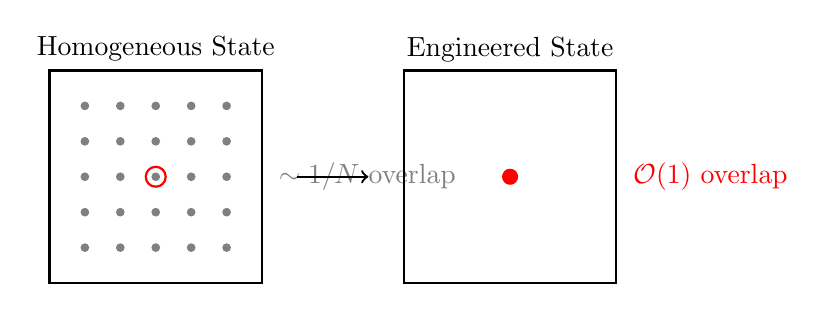
\begin{tikzpicture}[scale=0.9]
  % Left: Homogeneous
  \draw[thick] (0,0) rectangle (3,3);
  \node at (1.5, 3.3) {Homogeneous State};
  \foreach \x in {0.5, 1.0, ..., 2.5}
    \foreach \y in {0.5, 1.0, ..., 2.5}
      \filldraw[gray] (\x,\y) circle (1.5pt);
  \draw[red, thick] (1.5, 1.5) circle (4pt); % Target
  \node[right, gray] at (3.1, 1.5) {$\sim 1/N$ overlap};

  % Right: Engineered
  \draw[thick] (5,0) rectangle (8,3);
  \node at (6.5, 3.3) {Engineered State};
  \filldraw[red] (6.5, 1.5) circle (3pt); % Target
  \node[right, red] at (8.1, 1.5) {$\mathcal{O}(1)$ overlap};
  
  % Arrow
  \draw[->, thick] (3.5, 1.5) -- (4.5, 1.5);
\end{tikzpicture}
\caption{Degeneracy dilution. Left: In a homogeneous state, the selection operator $O_S$ (red circle) has small overlap with the $N$ equivalent embeddings. Right: In an engineered state, the pattern is pinned, yielding macroscopic overlap.}
\label{fig:dilution}
\end{figure}

\subsection{Structured states and pattern quality}
\label{sec:selection:structured}

In contrast, in a driven, mesoscopic, pattern-rich system (engineered materials, critical networks, biological tissues, etc.) the pattern encoded by $O_S$
can be realized in only a few places, and its overlap with the actual state can approach unity. We summarize this as
\begin{equation}
  \langle O_S\rangle \;\propto\; \mathcal{Q}\,\tilde{\Delta\Phi},
  \qquad
  0 \le \mathcal{Q} \le 1,
  \tag{5.5}
\end{equation}
where:
\begin{itemize}
  \item $\mathcal{Q}$ is a dimensionless \emph{pattern quality factor} (introduced more explicitly in Sec.~6), which measures how well the configuration matches the targeted pattern;
  \item $\tilde{\Delta\Phi}$ is a dimensionless free-energy difference associated with driving the system between two nearby macrostates in $S$.
\end{itemize}
The dependence on the structural distance $d_\sigma$ resides in the kernel $\Ksig = \exp[-d_\sigma/\lambda_\sigma]$ (Sec.~7). For large structural separations, $\Ksig\to 0$ and the coupling vanishes even if $\mathcal{Q}$ is high.

\subsection{Explicit example of a local $O_S$}

One convenient class of examples is based on a windowed functional of derivatives and curvature. Let $w_\ell(x)$ be a smooth, compactly supported window of linear size $\ell$, and define
\begin{equation}
  O_S(x)
  =
  \frac{1}{\Lambda^{\Delta-4}}
  \int d^4y\,\sqrt{-g(y)}\,
  w_\ell(x-y)\,
  \mathcal{F}\!\big(
    \nabla\phi(y),\,
    \nabla\nabla\phi(y),\,
    R_{\mu\nu\rho\sigma}(y)
  \big),
  \tag{5.6}
\end{equation}
with
\begin{equation}
  \mathcal{F}
  :=
  \sum_{m+n+k=\Delta} c_{mnk}\,
  \big(\nabla\phi\big)^{m}\,
  \big(\nabla\nabla\phi\big)^{n}\,
  \big(R_{\mu\nu\rho\sigma}\big)^{k},
  \tag{5.7}
\end{equation}
and coefficients $c_{mnk}$ chosen so that $O_S$ is scalar, gauge-invariant, and UV-soft above its design scale. The window function ensures locality on scales $\lesssim \ell$, while the polynomial structure makes $O_S$ sensitive to higher-order patterns (gradients, curvature, correlations) rather than just local field amplitudes.

Two genericity remarks are important here.  First, for a ``generic''
choice of coefficients $c_{mnk}$ (e.g.\ drawn from a broad, symmetric
distribution subject only to gauge invariance and UV softness), the
operator $O_S$ is highly sensitive to mesoscopic pattern structure but
its expectation value in homogeneous, periodic, or thermal states is
suppressed by degeneracy dilution.  If there are $N\gg 1$ macroscopically
equivalent ways of placing a given pattern inside such a state, then a
typical superposition of those placements yields
$\langle O_S\rangle \sim N^{-1/2}$ or smaller.  In the thermodynamic
limit this drives the quality factor $Q$ to zero.

Second, moving away from homogeneous states does not require fine
tuning of $c_{mnk}$.  Instead, one engineers platforms (Sec.~5.3) in
which the patterns singled out by $O_S$ are realized in only a few
locations with correlated phases (for example, near critical points or
edge-of-chaos regimes in complex networks).  In such states the overlap
with $O_S$ can approach order unity, $Q\sim 1$, while keeping the same
underlying definition of $O_S$.  In this sense the selection operator
is generic at the level of its field content; what is special is the
prepared state of the visible sector. All later constraints on the S-channel depend only on these generic properties of $O_S$---locality, symmetry, and degeneracy dilution---rather than on the particular choice of window function $w_\ell$ or polynomial $F$ in Eq.~(5.6).

\subsection{Why colliders see nothing}

Putting the pieces together, the effective contribution of Eq.~(5.1) to any collider observable schematically scales as
\begin{equation}
  \mathcal{A}_{\mathrm{collider}}
  \;\sim\;
  \varepsilon\,
  \langle O_S\rangle_{\mathrm{in}}\,
  \langle O_S\rangle_{\mathrm{out}}\,
  K_{\sigma,\mathrm{eff}},
  \tag{5.8}
\end{equation}
where ``in'' and ``out'' denote initial and final states in a high-energy experiment. For realistic beams and final states we expect:
\begin{itemize}
  \item approximate translational and rotational invariance;
  \item rapidly decorrelating phases;
  \item large degeneracy $N$ of equivalent pattern placements.
\end{itemize}
By the degeneracy-dilution argument (spelled out explicitly in the toy
model of Appendix~\ref{app:degeneracy-toy-model}), $\langle O_S\rangle_{\mathrm{in}}\approx
\langle O_S\rangle_{\mathrm{out}}\approx 0$ in such states, so that collider
cross-sections are suppressed by the \emph{state} rather than by RG
running. The same logic applies to cosmological and astrophysical plasmas that are nearly homogeneous on microscopic scales.

In summary, the selection operator $O_S$ is chosen so that:
\begin{itemize}
  \item it is technically natural and irrelevant in the Wilsonian sense (built from operators with $\Delta>4$ and normalized as in Eq.~(5.2));
  \item it has negligible expectation value in homogeneous, periodic, or thermal states due to degeneracy dilution;
  \item it can attain order-one values only in specially engineered, near-critical, pattern-rich systems, which are precisely the regimes targeted by our proposed experiments in Sec.~13.
\end{itemize}

\subsection{Radiative Stability via Pattern Sequestering}

A generic bilinear coupling between the visible sector and a Lorentz-violating substrate would typically induce dangerous lower-dimension operators (e.g., SME coefficients $\kappa_{JK}$) via vacuum loops. In standard EFT, these would be suppressed only by the coupling $\varepsilon$, leading to potential conflict with experimental bounds of order $10^{-18}$.

To resolve this, we introduce the \textbf{Pattern Sequestering Assumption}: the S-channel is not a universal modification of the vacuum, but a conditional channel active only in the presence of complex order.

We formalize this by treating the pattern-activation field $Q_*(x)$ introduced in Eq.~(3.1) as a background spurion. The interaction Lagrangian scales as:

\begin{equation}
\mathcal{L}_{int} \propto \varepsilon \, Q_*^2(x) \, O_S \, \chi
\end{equation}

This structure imposes specific constraints on radiative corrections:

\begin{enumerate}
\item \textbf{Vacuum Sequestering:} In the vacuum, homogeneous fluids, or standard collider environments used to define SME bounds, the pattern activation is negligible ($Q_* \equiv 0$). Consequently, the S-sector decouples entirely in these regimes. No S-induced Lorentz-violating operators are generated in the effective action for standard model fields in the vacuum background.

\item \textbf{Pattern Parity:} The $Q_*^2$ dependence is consistent with a discrete "Pattern Parity" symmetry ($Z_2^P$), under which $Q_* \to -Q_*$, $\chi \to -\chi$, and $O_S \to -O_S$, while visible fields remain even. This symmetry forbids all radiative corrections odd in the spurion, preventing linear leakage of Lorentz violation into the vacuum sector.

\item \textbf{Active Regime:} In the engineered systems targeted by experiments E1-E3, the spurion acquires a non-zero value $Q_* \sim \mathcal{Q}$, activating the channel. Radiative corrections in this regime are proportional to $\varepsilon Q^2$, which remains consistent with the phenomenological bounds discussed in Sec.~11.
\end{enumerate}

\emph{Loop-level scaling and SME coefficients.}---In a standard Wilsonian treatment, the interaction
\[
\mathcal{L}_{\rm int} \supset \varepsilon\,Q_*^2\,O_S\,\chi
\]
generates loop diagrams with two insertions of $\mathcal{L}_{\rm int}$ connected by $\chi$ and visible-field propagators. Schematically, a dimension-4 Lorentz-violating operator $\mathcal{O}_{\rm LV}$ in the visible sector (for example a photon-sector tensor contributing to $\tilde\kappa_{e-}$ in SME language) will appear with a coefficient of the form
\[
\delta c_{\rm LV} \sim \frac{(\varepsilon Q_*^2)^2}{16\pi^2}\,f\!\left(\frac{\Lambda}{\mu}\right),
\]
where $\Lambda$ is a UV cutoff for the effective description, $\mu$ is a renormalization scale, and $f$ is a dimensionless loop function of order unity. In homogeneous or vacuum backgrounds we set $Q_*\equiv 0$, so these coefficients vanish identically at any loop order: there is no radiative leakage of Lorentz violation into the vacuum EFT. In an engineered high-$Q$ configuration one has $Q_*\sim Q\ll 1$, so that induced coefficients scale at least as $\varepsilon^2 Q^4$. For benchmark values $\varepsilon\lesssim 10^{-15}$ and ambitious targets $Q\lesssim 10^{-2}$, this places loop-generated photon-sector coefficients safely below the existing bounds discussed in Sec.~11 even if the S-channel comes close to saturating the thermodynamic resource inequality.

A complete multi-loop matching calculation to the full SME parameter set would require specifying a UV completion of the S-sector and is beyond the scope of this work. What we rely on in this paper is the structural statement that every Lorentz-violating operator in the visible-only EFT carries at least two powers of $Q_*$ and therefore vanishes in the homogeneous and vacuum regimes where current SME bounds are obtained.

This sequestering mechanism turns the radiative stability problem into a structural statement about the substrate: the pattern-local channel is strictly conditional on the presence of active pattern complexity.

\section{Coupling Strength and Dimensional Analysis}

At the level of coarse-grained phenomenology it is convenient to express the substrate flow as a scalar power assigned to each active edge or calibrated pair $e$ in the experimental setup. We denote this by $\Psig(e)$ to stress that it is a scalar \emph{power} (units of W), distinct from the 4-current $\Jsig$ appearing in the covariant conservation equations.

\subsection{Power form}

We parameterize the power flowing into the $S$-sector along edge $e$ as
\begin{equation}
  \Psig(e)
  \;=\;
  \varepsilon\,
  \Ksig(e)\,
  \mathcal{Q}(e,t)\,
  \Delta\tilde{\Phi}(e)\,
  P_{\mathrm{pump}}(e)
  \quad\text{(units: W)},
  \tag{6.1}
\end{equation}
where:
\begin{itemize}
  \item $\varepsilon$ is the dimensionless microscopic coupling strength entering the interaction Lagrangian;
  \item $\Ksig(e)=\exp[-d_\sigma(e)/\lambda_\sigma]$ is the dimensionless similarity factor for edge $e$, constructed from the $d_\sigma$-metric of Sec.~7;
  \item $\mathcal{Q}(e,t)\in[0,1]$ is a dimensionless pattern quality factor for that edge at time $t$;
  \item $\Delta\tilde{\Phi}(e)$ is a dimensionless free-energy increment associated with the driven transition on edge $e$;
  \item $P_{\mathrm{pump}}(e)$ is the physical pump power (in W) available to drive the transition.
\end{itemize}
By construction, the right-hand side has dimension of power, so Eq.~(6.1) is dimensionally consistent.

\subsection{Rate form}

It is often convenient to re-express the pump in terms of a rate. For a characteristic quantum $\hbar\omega_0$ of the driven transition, define
\begin{equation}
  \PumpRate(e)
  :=
  \frac{P_{\mathrm{pump}}(e)}{\hbar\omega_0}
  \quad [\mathrm{s^{-1}}],
\end{equation}
so that Eq.~(6.1) can be written as
\begin{equation}
  \Psig(e)
  =
  \varepsilon\,
  \hbar\omega_0\,
  \Ksig(e)\,
  \mathcal{Q}(e,t)\,
  \PumpRate(e)\,
  \Delta\tilde{\Phi}(e).
  \tag{6.2}
\end{equation}
This form will be useful when connecting to the thermodynamic and information-theoretic bounds in Sec.~8.

\subsection{Degeneracy dilution and state dependence}

The factor $\mathcal{Q}(e,t)$ encodes how well the actual microscopic configuration on edge $e$ matches the high-complexity pattern selected by $O_S$. As discussed in Sec.~5, in homogeneous or periodic systems there are many equivalent placements of the same pattern. If there are $N$ such placements, the overlap between the actual state and the specific pattern singled out by $O_S$ scales as $1/\sqrt{N}$, so that
\[
|\langle O_S\rangle|^2 \sim \frac{1}{N}.
\]
In the thermodynamic limit $N\to\infty$ this implies $\mathcal{Q}\to 0$ and hence
\begin{equation}
  \Psig(e) \to 0
  \qquad
  \text{(homogeneous / thermal / periodic states)}.
  \tag{6.3}
\end{equation}
This is the precise sense in which aether resonance is absent in ordinary matter: even if $\varepsilon$ is not extremely small, $\mathcal{Q}$ is effectively zero, and no appreciable power flows into the $S$-sector.

Conversely, in carefully engineered, mesoscopic, pattern-rich or near-critical systems the number of equivalent placements can be $\mathcal{O}(1)$, and $\mathcal{Q}$ can approach unity. Then $\Psig(e)$ can be an appreciable fraction of $P_{\mathrm{pump}}(e)$ (further bounded by thermodynamics in Sec.~8). This is the regime targeted by experiments E1--E3.

\section{Operationalized $d_\sigma$-Metric}

Algorithmic similarity between two microscopic configurations is in general non-computable. For phenomenology and experiment design we therefore introduce a \textbf{practical proxy} for the structural distance $d_\sigma$ and the associated similarity factor $\Ksig$.

\subsection{Feature embedding and surrogate distance}

We associate to each substrate configuration $\sigma\in S$ a finite-dimensional feature vector
\[
\mathcal{I}(\sigma)
=
\big(\mathcal{I}_1(\sigma),\ldots,\mathcal{I}_{N_{\mathrm{feat}}}(\sigma)\big),
\]
where the components $\mathcal{I}_I$ are chosen to be:
\begin{itemize}
  \item invariant under gauge transformations and diffeomorphisms in $M$;
  \item local or quasi-local in the emergent spacetime (e.g.\ power spectra, correlation functions, topological descriptors);
  \item experimentally accessible in principle (e.g.\ from probe measurements, imaging, or electrical response).
\end{itemize}
Given positive weights $w_I>0$ and an embedding scale $\ell_0$, we define
\begin{equation}
\begin{split}
  d_\sigma(\sigma,\sigma')
  &:= \ell_0\,
  \left(
    \sum_{I=1}^{N_{\mathrm{feat}}}
      w_I\,
      \big\|
        \mathcal{I}_I(\sigma)
        -\mathcal{I}_I(\sigma')
      \big\|^2
  \right)^{1/2},
  \\
  \Ksig(\sigma,\sigma')
  &\equiv
  \exp\!\big[-d_\sigma(\sigma,\sigma')/\lambda_\sigma\big].
\end{split}
\tag{7.1}
\end{equation}
This construction makes $d_\sigma$ a bona fide metric on $S$ (up to equivalence of configurations with identical feature vectors) and implements the exponential falloff assumed in the mediator kernel.

\subsection{Choice of features}

The specific choice of features is not unique and can be adapted to the experimental platform. Examples include:
\begin{itemize}
  \item local Fourier spectra or wavelet coefficients (capturing periodicity and band structure);
  \item two-point and higher-order correlators (capturing spatial organization and long-range order);
  \item topological descriptors (e.g.\ Betti numbers from persistent homology of level sets of a field);
  \item response functions (e.g.\ impedance spectra, transfer functions of neural or electronic circuits).
\end{itemize}
The scale $\ell_0$ sets the typical size of $d_\sigma$ for a ``unit'' change in features. In practice, we will choose $\ell_0$ and $\lambda_\sigma$ such that a qualitatively clear change in the pattern (e.g.\ block-scrambling or strong noise) corresponds to $d_\sigma \sim \lambda_\sigma$, while minor modifications (e.g.\ global phase rotations) yield $d_\sigma\ll\lambda_\sigma$.

\subsection{Distance ladder for calibration}

To connect the abstract $d_\sigma$ to observable quantities, we introduce a \textbf{distance ladder}: a set of calibrated transformations labelled by an integer level $\ell=0,\ldots,5$ applied to a reference pattern $s$, producing configurations $s_\ell$. For each level we measure or infer a typical structural distance $\varepsilon_\ell:=d_\sigma(s,s_\ell)$ and the corresponding similarity $K_{\sigma,\ell}:=\exp[-\varepsilon_\ell/\lambda_\sigma]$.

An illustrative ladder is:

\begin{table}[t]
\centering
\begin{tabular}{@{}c l c c@{}}
\toprule
Level $\ell$ & Transformation & $d_\sigma$ scale & $K_{\sigma,\ell}$ \\
\midrule
0 & Identical $(s' = s)$ & $0$ & $1$ \\
1 & Phase rotation (spectrum preserved) & $\varepsilon_1 \ll \lambda_\sigma$ & $\approx 0.9$ \\
2 & Permuted label / mild relabelling & $\varepsilon_2 \approx 0.3\,\lambda_\sigma$ & $\approx 0.7$ \\
3 & Block-scramble (temporal/spatial) & $\varepsilon_3 \approx 0.7\,\lambda_\sigma$ & $\approx 0.5$ \\
4 & Additive noise (SNR $=10$ dB) & $\varepsilon_4 \approx \lambda_\sigma$ & $\approx 0.37$ \\
5 & Independent realization & $\varepsilon_5 \gg \lambda_\sigma$ & $\ll 0.1$ \\
\bottomrule
\end{tabular}
\end{table}

In practice, the values in the last two columns are not assumed but \emph{measured} (or inferred) by running the full experimental protocol with controlled pattern distortions. The ladder then provides a direct, empirical link between:
\begin{itemize}
  \item observable changes in the experimental pattern;
  \item the corresponding change in $d_\sigma$;
  \item the decay of the effect through the factor $\Ksig=\exp[-d_\sigma/\lambda_\sigma]$.
\end{itemize}

\subsection{Pre-registration}

For the proposed experiments E1--E3 we envisage pre-registering the distance ladder as part of the analysis plan:
\begin{itemize}
  \item the transformations corresponding to each level $\ell$ are fixed in advance and implemented blindly (e.g.\ by a separate team or by automated code);
  \item the ladder is used to fit or constrain $\lambda_\sigma$ by comparing the observed effect size at each level with the expected $\exp[-d_\sigma/\lambda_\sigma]$ falloff;
  \item the mapping between level labels and transformation details is kept sealed until after the primary analysis to avoid experimenter bias.
\end{itemize}
This operationalizes the otherwise abstract notion of $d_\sigma$ in a way that can be compared directly to data.

\section{Thermodynamics and Measurable Cost}

We now connect the phenomenological power $\Psig$ to thermodynamic and information-theoretic constraints. The key idea is that any reliable transfer of information through the $S$-channel requires the production of entropy in the combined system, and that a finite pump power therefore bounds the achievable FTL bitrate.

\subsection{Pattern free energy}

We define an effective \textbf{pattern free energy} for the $S$-sector,
\begin{equation}
  \mathcal{F}_S
  =
  \langle E_S \rangle - \Temp\,\Sigma_S,
  \tag{8.1}
\end{equation}
where $\Sigma_S$ is an entropy-like functional of the microscopic $S$-state (e.g.\ approximated by minimum description length or compression ratio) and $\Temp$ is an effective temperature associated with the degrees of freedom that the pump can thermalize. In the spirit of Landauer's principle, we will require that each reliably distinguishable bit communicated through the $S$-channel carries a minimal entropy cost~\cite{landauer1961_irreversibility,berut2012_landauer_exp,jun2014_landauer_precision}.

\subsection{Minimal Markov model on S-edges}

We model each active $S$-edge $e$ as a two- or few-state Markov process driven by the pump. The edge switches between microstates $\{i\}$ with transition rates $k_{ij}(t)$ that depend on the external driving. Standard stochastic thermodynamics then associates to each realization:
\begin{itemize}
  \item a stochastic entropy production $\Delta S_{\mathrm{tot}}(e)$;
  \item a heat $Q_{\mathrm{diss}}(e)$ dumped into the environment;
  \item a Kullback--Leibler divergence $D_{\mathrm{KL}}$ between the forward and time-reversed trajectory ensembles.
\end{itemize}
Results due to Crooks, Seifert, and others imply a general inequality
\begin{equation}
  \langle \Delta S_{\mathrm{tot}} \rangle
  \;\ge\;
  k_B\,D_{\mathrm{KL}}(\mathrm{forward}\|\mathrm{backward}),
  \tag{8.2}
\end{equation}
with $\langle\cdot\rangle$ denoting an ensemble average. When the dynamics is used to transmit an average of $I_e$ bits of information along edge $e$, the KL divergence satisfies
\[
  D_{\mathrm{KL}} \;\ge\; I_e \ln 2,
\]
so we obtain a Landauer-type inequality
\begin{equation}
  \langle Q_{\mathrm{diss}}(e)\rangle
  \;\ge\;
  k_B \Temp \ln 2 \cdot I_e,
\end{equation}
i.e.\ at least $k_B \Temp \ln 2$ of dissipated heat per reliably transmitted bit.

\subsection{Resource inequality for FTL bitrate}

Let $R_{\mathrm{bit}}(e)$ be the average bit rate (bits per second) transmitted along the $S$-channel for edge $e$ in a stationary regime, and let $P_{\mathrm{diss}}(e)$ be the average rate of heat dissipation that can be used for signalling. From the inequality above we obtain
\begin{equation}
  R_{\mathrm{bit}}(e)
  \;\le\;
  \frac{P_{\mathrm{diss}}(e)}{k_B \Temp \ln 2}.
\end{equation}
Not all of the pump power is available for structured signalling. We therefore set
\begin{equation}
  P_{\mathrm{diss}}(e)
  =
  \beta\,
  \Psig(e),
\end{equation}
where $0<\beta\le 1$ collects inefficiencies in the conversion from pump work to low-entropy pattern changes that actually carry information (e.g.\ losses to uncontrolled degrees of freedom). Using Eq.~(6.1) for $\Psig(e)$, we obtain
\begin{equation}
  R_{\mathrm{bit}}(e)
  \;\le\;
  \frac{\beta}{k_B \Temp \ln 2}\,
  \varepsilon\,
  \Ksig(e)\,
  \mathcal{Q}(e,t)\,
  \Delta\tilde{\Phi}(e)\,
  P_{\mathrm{pump}}(e).
  \tag{8.3}
\end{equation}
\textbf{This is the central bound of the paper.} Equation~(8.3) is the thermodynamic \emph{resource inequality} that underpins all subsequent predictions and experimental design: for fixed pump power and temperature, the achievable FTL bit rate is bounded by the product of the microscopic parameters $(\varepsilon,\Ksig,\mathcal{Q},\tilde{\Delta\Phi})$. In particular, for a given experimental platform, a null result in a carefully designed protocol directly constrains combinations of these parameters.

\subsection{Bounding parameters from null results}

Suppose an experiment of type E1 yields a null result in the sense that no FTL signal is detected above a bit-rate threshold $R_{\mathrm{bit}}^{(\mathrm{null})}$ for a given edge and pump configuration. Taking $\tilde{\Delta\Phi}\le 1$ as a conservative assumption (i.e.\ the free-energy difference per operation does not exceed $k_B\Temp$), Eq.~(8.3) implies
\begin{equation}
  \varepsilon\,\mathcal{Q}\,e^{-d_\sigma/\lambda_\sigma}
  \;<\;
  \frac{k_B \Temp \ln 2}{\beta\,P_{\mathrm{pump}}}\,
  R_{\mathrm{bit}}^{(\mathrm{null})}.
  \tag{8.4}
\end{equation}
In a regime where $\varepsilon$ is independently constrained (for example by photon-sector tests or SME bounds), Eq.~(8.4) can be interpreted as a direct bound on the product $\mathcal{Q}\,e^{-d_\sigma/\lambda_\sigma}$, with $d_\sigma$ calibrated using the distance ladder of Sec.~7. Conversely, if an effect is observed and cross-checked against multiple protocols, Eq.~(8.3) provides a consistency relation between the inferred parameters.

Taken together with the energetic constraints from E2 (Sec.~12) and the anisotropy bounds from photon-sector tests, the thermodynamic inequality in Eq.~(8.3) helps carve out a small, sharply defined region of parameter space where aether resonance could reside.

\section{Modified Lieb-Robinson Bound}

In standard local quantum lattice systems, the Lieb--Robinson bound states that the commutator of two observables $A(x,t)$ and $B(y,0)$ supported near spatial points $x,y\in M$ is exponentially suppressed outside an effective light cone:
\[
  \|[A(x,t),B(y,0)]\|
  \;\lesssim\;
  C\,\exp\!\big[-\kappa(|x-y|-v t)\big],
\]
for some constants $C,\kappa>0$ and maximal group velocity $v$.

\subsection{Including S-edges}

In our framework there are additional, substrate-mediated couplings. Let $E_S$ be the set of active $S$-edges, and for each edge $e=(\sigma,\sigma')$ we include a weak Hamiltonian perturbation
\[
  \delta H_S
  =
  \sum_{e\in E_S} h_e,
\]
where $\|h_e\|\le \eta$ and the edges connect microscopic degrees of freedom whose projections in $M$ may be far apart. The structural distance and similarity enter via the kernel
\[
  \|h_e\|
  \;\propto\;
  e^{-d_\sigma(\sigma,\sigma')/\lambda_\sigma},
\]
and the substrate graph has bounded degree $g$ (each node participates in at most $g$ edges). The mediator field propagates through $S$ at finite speed $c_S$.

\subsection{Soft cone with S-damping}

Under the technical assumptions listed in Appendix~C (bounded operator norms, finite propagation speed $c_S$ in $S$, exponential kernel decay with rate $\mu$, and weak coupling $\eta$ such that $\mu>\ln g$; see particularly Assumptions~A3 and A5 in Appendix~E), one can prove the following modified bound.

\begin{lemma}[Soft cone with S-damping]
There exist constants $C,C',\kappa>0$ and $v$ such that, for all local observables $A(x,t)$ and $B(y,0)$,
\begin{equation}
\begin{split}
  \big\|[A(x,t),B(y,0)]\big\|
  &\le
  C\,e^{-\kappa(|x-y|-v t)}
  \\
  &\quad
  +\;
  C'\,
  \Theta\!\big(t-\tfrac{d_\sigma(\sigma_x,\sigma_y)}{c_S}\big)\,
  e^{-d_\sigma(\sigma_x,\sigma_y)/\lambda_\sigma}\,
  \Phi\!\left(g,\frac{\eta t}{\hbar}\right),
\end{split}
\tag{9.1}
\end{equation}
where $\sigma_x,\sigma_y\in S$ are substrate representatives of the regions around $x$ and $y$, $\Theta$ is the Heaviside step function, and
\begin{equation}
  \Phi\!\left(g,\frac{\eta t}{\hbar}\right)
  :=
  \exp\!\big[g\,e^{-\mu}\,\eta t/\hbar\big] - 1.
  \tag{9.2}
\end{equation}
\end{lemma}

The first term in Eq.~(9.1) is the usual Lieb--Robinson light-cone contribution with effective velocity $v$ close to $c$. The second term encodes the substrate-mediated tail: it vanishes for times $t<d_\sigma(\sigma_x,\sigma_y)/c_S$ (no effect can propagate through $S$ faster than $c_S$) and is exponentially suppressed in the structural distance $d_\sigma$.

\subsection{Sketch of proof}

The detailed proof is given in Appendix~C; here we summarize the structure.

\paragraph{1. Duhamel expansion.}
We write the full time evolution in the interaction picture with respect to the ``bare'' Hamiltonian $H_M$ on $M$ and treat $\delta H_S$ as a perturbation. Iterating the Duhamel formula yields an expansion in the number of $S$-mediated hops, schematically
\[
  A(t)
  =
  A_M(t)
  +
  \frac{i}{\hbar}
  \int_0^t ds\,U^\dagger(t,s)\,[\delta H_S(s),A_M(s)]\,U(t,s)
  + \cdots ,
\]
where $A_M(t)$ is the Heisenberg evolution under $H_M$ alone and $U(t,s)$ is the evolution operator with the perturbation included.

\paragraph{2. Commutator growth.}
Bounding the norm of nested commutators with the local pieces $h_e$ along a path of $n$ $S$-edges gives a factor
\[
  \big\|[h_{e_n},[h_{e_{n-1}},\ldots,[h_{e_1},A_M]\ldots]]\big\|
  \;\le\;
  (2\eta)^n \|A\|.
\]
Summing over all such paths with at most $g$ outgoing edges per node introduces a combinatorial factor $\sim g^n$.

\paragraph{3. Kernel suppression and average distance.}
Each substrate hop contributes a factor $e^{-\mu}$, where $\mu$ is the dimensionless decay rate of the kernel in $S$. Along a path connecting $\sigma_x$ and $\sigma_y$ with $n$ hops, the total damping is roughly $e^{-\mu n}$, which can be related to $e^{-d_\sigma(\sigma_x,\sigma_y)/\lambda_\sigma}$ when $d_\sigma$ is extensive along paths. The effective average damping per hop is $\exp(-\mu)$.

\paragraph{4. Sum over paths and convergence.}
Collecting the factors from steps 2 and 3 and summing over $n$ leads to the function
\[
  \Phi\!\left(g,\frac{\eta t}{\hbar}\right)
  =
  \sum_{n\ge 1}
    \frac{1}{n!}
    \big( g e^{-\mu} \eta t/\hbar \big)^n
  =
  \exp\!\big[g e^{-\mu} \eta t/\hbar\big] - 1,
\]
which converges provided $g e^{-\mu}<1$. This is precisely the sparsity condition assumed in Appendix~C. Importantly, $\Phi$ does not saturate to a distance-independent constant; the exponential factor $e^{-d_\sigma/\lambda_\sigma}$ remains in front.

\paragraph{5. Retardation.}
Finally, each hop in $S$ is associated with a finite propagation speed $c_S$. This yields a Heaviside factor $\Theta(t-d_\sigma/c_S)$ when bounding the integrals over intermediate times in the Duhamel expansion: the substrate-mediated tail cannot contribute before the mediator has had time to traverse the structural distance between $\sigma_x$ and $\sigma_y$.

\subsection{Causal interpretation}

The bound in Eq.~(9.1) shows that, even with $S$-mediated couplings, there is no instantaneous, distance-independent commutator outside the emergent light cone. Instead, there is a ``soft cone'' inside which correlations can be enhanced by substrate effects, but always subject to:
\begin{itemize}
  \item exponential decay in structural distance $d_\sigma$;
  \item retardation at speed $c_S$ in $S$;
  \item smallness controlled by sparsity $g$ and weak coupling $\eta$.
\end{itemize}
In particular, the combination of this bound with the category-theoretic anti-telephone argument (Sec.~10) excludes paradoxical closed causal loops: superluminal transfer in $M$ is compatible with a globally well-defined causal order in $T$ and $S$.

\section{Causality – Formal Proof}

In this section we make precise what is meant by ``causal'' in the presence of substrate-local FTL transfer and prove that the framework excludes closed causal loops and antitelephone constructions.

\subsection{Monotonic substrate time}

The substrate dynamics comes with a global discrete update parameter $T=0,1,2,\dots$ and a coarse-grained \emph{substrate time function} $\tau$ which is strictly monotonically increasing along any physically allowed microscopic transition. We summarize this as:

\textbf{Monotonic-$(T)$ axiom:} For every elementary substrate transition
\[
  (s,T)\longrightarrow (s',T')
\]
with nonzero amplitude, the associated substrate time increment satisfies
\begin{equation}
  \Delta \tau := \tau(s',T') - \tau(s,T) > 0,
  \qquad
  \text{all kernels are retarded in $T$}.
  \tag{10.1}
\end{equation}
In particular, the mediator kernel $G_{\rm ret}$ in $S$ (Sec.~4) vanishes for $T'<T$, and all effective kernels in $M$ obtained by integrating out $S$ inherit this retardation.

\subsection{Events as objects in a causal category}

We formalize the causal structure on $M\times S$ using the language of categories, following standard approaches in algebraic quantum field theory.

\begin{itemize}
\item \textbf{Objects:} Localized events $e$, i.e.~equivalence classes of microscopic configurations supported in small regions of $M\times S$ together with a finite interval of substrate time $\tau$.
\item \textbf{Morphisms:} A morphism $f:e\to e'$ is a physically allowed influence chain produced by composing:
  \begin{enumerate}
    \item local evolution in $M$ generated by the visible-sector Hamiltonian $H_M$;
    \item substrate-mediated hops through $S$ via the $S$-mediator and selection operator $O_S$;
    \item classical communication constrained to future light cones in $(M,g)$.
  \end{enumerate}
\end{itemize}

Composition of morphisms is concatenation of influence chains. By construction, every elementary piece of a morphism is retarded in substrate time and respects the Monotonic-$(T)$ axiom.

Define a functor
\[
  \mathcal{T}:\mathcal{C}\to(\mathbb{R},\le)
\]
from the causal category $\mathcal{C}$ to the totally ordered set of real numbers, by assigning to each event $e$ the minimal substrate time $\tau(e)$ at which it can occur and to each morphism $f:e\to e'$ the increment
\[
  \mathcal{T}(f)=\tau(e')-\tau(e).
\]
By the Monotonic-$(T)$ axiom, $\mathcal{T}(f)>0$ for every non-identity morphism $f$.

\begin{theorem}[Causal monotonicity]
Under the assumptions that (i) all microscopic rules are retarded in substrate time and satisfy $\Delta\tau>0$ as in Eq.~\textup{(10.1)}, (ii) the $S$-mediator has finite propagation speed $c_S$ and exponential damping in $d_\sigma$ (Sec.~9), and (iii) every macroscopic process is built from a finite concatenation of such microscopic transitions, there exist no closed causal loops in $(M\times S)$.
\end{theorem}

\begin{proof}[Sketch]
Suppose for contradiction that there exists a nontrivial closed loop in $\mathcal{C}$, i.e.~a morphism $f:e\to e$ which is not the identity. Functoriality of $\mathcal{T}$ implies
\[
  \mathcal{T}(f\circ f) = \mathcal{T}(f) + \mathcal{T}(f).
\]
Iterating, for $n$ copies we obtain $\mathcal{T}(f^{\circ n}) = n\,\mathcal{T}(f)$. On the other hand, by the Monotonic-$(T)$ axiom every non-identity morphism has strictly positive substrate time length, so $\mathcal{T}(f)>0$. This is incompatible with $f$ being a loop based at $e$, because by definition a causal loop must return to the same event at the same substrate time, which would require $\mathcal{T}(f)=0$. Hence no such nontrivial loop exists. \qedhere
\end{proof}

The technical assumptions (ii) and (iii) ensure that the effective evolution on $M$ inherits a generalized Lieb--Robinson bound with a soft cone (Sec.~9) and that the category $\mathcal{C}$ is well-defined.

\subsection{Anti-telephone rule}

We now formulate the operational rule that forbids antitelephone constructions.

\textbf{Rule (anti-telephone):} A substrate-mediated transfer between two laboratories $A$ and $B$ is only permitted if each microscopic resonance step in the chain satisfies
\begin{equation}
  \Delta\tau > 0
\end{equation}
in the substrate frame. Chains that would require $\Delta\tau<0$ for any microscopic step are assigned zero amplitude.

This rule is local in $(M\times S)$: it is enforced at the level of individual resonance events and does not depend on the global motion of the laboratories. Because $\tau$ is a scalar time function on the substrate, it is the same for all inertial observers in $M$.

\begin{corollary}[Two-lab antitelephone exclusion]
Consider two laboratories $A$ and $B$ following arbitrary timelike worldlines in $(M,g)$ with four-velocities $U_A^\mu$ and $U_B^\mu$. Assume each laboratory can use a combination of subluminal signals in $M$ and substrate-local resonance steps in $S$. Under the Monotonic-$(T)$ axiom and the anti-telephone rule above, there exists no protocol by which $A$ and $B$ can arrange for a message to arrive at the sender's own past proper time.
\end{corollary}

\begin{proof}[Sketch]
Any protocol can be decomposed into a finite sequence of morphisms in $\mathcal{C}$ corresponding to local operations at $A$ or $B$, subluminal communications in $M$, and resonance steps in $S$. The functor $\mathcal{T}$ assigns to each such morphism a strictly positive time increment, because local operations and subluminal signals are future-directed in $(M,g)$ and resonance steps obey $\Delta\tau>0$. Therefore the total substrate time elapsed along the protocol is strictly positive as seen by both laboratories, and no closed causal loop in the sense of proper time is possible. \qedhere
\end{proof}

\subsection{Relation to the Lieb–Robinson bound}

Section~9 established a modified Lieb--Robinson inequality, Eq.~(9.1), which bounds the norm of commutators of local observables outside an effective light cone and shows that substrate-mediated effects produce only a soft tail exponentially suppressed in $d_\sigma$ and retarded by $c_S$ in $S$. Combining that bound with the categorical argument above yields:

\begin{itemize}
\item No exact, instantaneous commutators at spacelike separation in $M$; the commutator norm remains exponentially small outside the soft cone.
\item No possibility of closed causal curves in $(M\times S)$, because every influence chain has strictly positive $\Delta\tau$.
\end{itemize}

\textbf{Conclusion.} The model permits FTL transfer in the emergent spacetime $(M,g)$ while maintaining a globally well-defined causal order in substrate time. The combination of the Monotonic-$(T)$ axiom, the anti-telephone rule, and the modified Lieb--Robinson bound rules out antitelephone paradoxes.

\section{Compatibility with Established Tests and Anisotropy Budget}

The framework must be consistent with the very tight constraints on Lorentz violation and preferred-frame effects coming from Michelson--Morley, Hughes--Drever, resonant-cavity, and astrophysical tests. In this section we sketch how the aether-resonance phenomenology maps onto standard parametrizations and define an ``anisotropy budget'' that will later be compared to experimental sensitivities.

\subsection{Anisotropy from a preferred substrate frame}

In the substrate rest frame there is a distinguished timelike unit vector
\[
  \xi^\mu = (1,0,0,0),
\]
which induces small preferred-frame corrections in the dispersion relations of particles and photons once the $S$-mediated coupling is taken into account. At leading order one can write for a particle of mass $m$ and momentum $p^\mu$:
\begin{equation}
    E^2 = p^2 c^2 + m^2 c^4\,\big[1+\Delta(E,\hat p\!\cdot\!\hat\xi)\big],
    \tag{11.1}
\end{equation}
with $\hat p$ the unit vector along the spatial momentum and $\Delta$ a dimensionless modifier.

For concreteness, we parametrize the leading anisotropic contribution as
\begin{equation}
    \Delta \;\sim\; \varepsilon\left(\frac{\lambda_\sigma}{\lambda_C}\right)\mathcal Q
    \left(\frac{E}{mc^2}\right)\,(\hat p\!\cdot\!\hat\xi)^2,
    \tag{11.2}
\end{equation}
where $\lambda_C=\hbar/(mc)$ is the Compton wavelength associated with the relevant degree of freedom, $\lambda_\sigma$ is the structural range of the $S$-kernel, and $\mathcal Q$ is an appropriate quality factor ($\Qgam$ for photons, $\Qmat$ for matter). Equation~(11.2) should be understood as an order-of-magnitude scaling rather than a precise prediction; its purpose is to connect the microscopic parameters $(\varepsilon,\lambda_\sigma,\mathcal Q)$ to effective anisotropies.

For photons $(m=0)$, it is convenient to rewrite the result in terms of an effective anisotropic modification of the speed of light. Taking $E=pc$ and using a representative microscopic scale in place of $\lambda_C$, one finds
\begin{equation}
    \frac{\Delta c}{c} \;\sim\; \epsgam\left(\frac{\lsig}{\lambda_C}\right)\Qgam,
    \tag{11.3}
\end{equation}
where $\epsgam$ denotes the photon-sector coupling, $\lsig$ the effective structural range relevant for the optical mode, and $\Qgam$ the photon-sector quality factor.

\subsection{Photon-sector SME parametrization}

In the photon sector, Lorentz-violating effects are conventionally expressed using the Standard-Model Extension (SME) in terms of the matrices $\tilde\kappa_{e-}^{JK}$, $\tilde\kappa_{o+}^{JK}$, and the scalar $\tilde\kappa_{\rm tr}$. To leading order, the aether-resonance model produces a traceless, symmetric contribution of the form
\begin{equation}
\tilde\kappa_{e-}^{JK}\ \sim\ \epsgam\,\Qgam\,
\Big(\frac{\lsig}{L_{\rm exp}}\Big)\,\Xi^{JK},
\end{equation}
where $L_{\rm exp}$ is a characteristic size of the optical apparatus and $\Xi^{JK}=\mathcal{O}(1)$ is a geometry-dependent tensor encoding its orientation with respect to $\hat\xi$.

State-of-the-art cavity and clock-comparison experiments bound the relevant components of $\tilde\kappa_{e-}^{JK}$ at roughly the $10^{-18}$ level or better. Translating Eq.~(11.3) into this language and comparing gives
\begin{equation}
    \epsgam\left(\frac{\lsig}{\lambda_C}\right)\Qgam \;\lesssim\; 10^{-18}.
    \tag{11.4}
\end{equation}
For illustration, taking $\lsig \sim 1\,\mu{\rm m}$ and a representative microscopic scale $\lambda_C \sim 10^{-12}\,{\rm m}$ (so that $\lsig/\lambda_C \sim 10^6$) implies
\[
  \epsgam \Qgam \lesssim 10^{-24}.
\]
Given that $0\le \Qgam\le 1$, this bound can be interpreted as a strong constraint on the photon-sector coupling $\epsgam$, independently of the details of $O_S$.

\subsection{Daily/annual modulation and anisotropy budget}

Because the Earth rotates and orbits relative to the substrate rest frame, any preferred-frame effect will generally produce sidereal and annual modulations in observables. In the photon sector this is captured by the usual SME analysis of cavity experiments. In the matter sector, where direct bounds are much weaker, we can parameterize the sidereal modulation amplitude $A_{\rm sid}^{(\mathrm{mat})}$ in the E2-type setups of Sec.~12 by
\[
A_{\rm sid}^{(\mathrm{mat})} \simeq \epsmat \left( \frac{\lsig}{L_{\rm exp}} \right) \Qmat \, \Xi,
\]
where $\epsmat$ and $\Qmat$ are the matter-sector coupling and quality factor, $L_{\rm exp}$ is the size of the macroscopic apparatus, and $\Xi=\mathcal{O}(1)$ encodes geometrical factors and projection onto the rotation axis.

We will return to a more detailed phenomenological expression in Eq.~(12.4), where $A_{\rm sid}^{(\mathrm{mat})}$ is related directly to the ratio of matter- and photon-sector parameters. For now it is sufficient to note that:
\begin{itemize}
  \item Photon-sector tests tightly constrain the combination $\epsgam(\lsig/\lambda_C)\Qgam$ via Eq.~(11.4).
  \item Matter-sector sidereal modulation in E2 provides a direct empirical handle on $\epsmat (\lsig/L_{\rm exp})\Qmat$.
\end{itemize}
The ``anisotropy budget'' is the requirement that both sectors can be made simultaneously consistent with these bounds and with any positive signal in the proposed experiments.

\section{Predictions and Numerical Targets}

We summarize the qualitative and quantitative predictions of the framework in a form suitable for comparison with existing and future experiments.

\textbf{Negative predictions (should not be seen):}

\begin{itemize}
\item No deviations from tested gravitational laws, no observable vacuum dispersion, and no anomalous signals in torsion-balance or gravitational-wave experiments. The metric sector remains governed by standard GR with $\alpha\equiv 1$; aether resonance affects only the distribution of stress--energy, not the gravitational coupling.
\item No robust effects in homogeneous crystals or fluids: in the limit $N\gg 1$ equivalent placements of a pattern, degeneracy dilution drives the pattern quality factor $\mathcal Q\to 0$ so that $\Psig\to 0$ (Sec.~5--6).
\item No signals in accelerator experiments: beams and final states are approximately translationally invariant and thermal on microscopic scales, implying $\langle O_S\rangle_{\rm in}\approx\langle O_S\rangle_{\rm out}\approx 0$ even though the seed operator is built from irrelevant operators with $\Delta>4$ (Sec.~5.3). Collider cross-sections therefore receive negligible contributions from the $S$-channel.
\item No everyday signalling without shared structure and pump: in the absence of deliberately engineered, high-$\mathcal Q$ patterns and nontrivial pump power $P_{\rm pump}$, Eq.~(6.1) forces $\Psig\approx 0$.
\end{itemize}

\textbf{Positive predictions with numerical targets:}

\subsection{Pred.\ 1: Twin-reservoir correlations (E1)}

\textbf{Goal.} A statistically significant reduction in bit error rate (BER) between two spacelike-separated reservoirs that share structure in $S$ and are both driven by high-quality pumps, compared to carefully matched control configurations that differ only in the pattern features entering $O_S$. Such reservoirs can be implemented using physical reservoir computing architectures, including photonic and electronic reservoirs, which are known to provide high-dimensional dynamical feature maps for complex input patterns~\cite{tanaka2019_physical_reservoir,vandersande2017_photonic_reservoir}.

Specializing the thermodynamic resource inequality (8.3) to the E1 setup gives an upper bound on the achievable FTL bit rate per edge $e$,
\[
  R_{\rm bit}(e)
  \;\le\;
  \frac{\beta}{k_B T \ln 2}\,
  \varepsilon\,\Ksig(e)\,\mathcal Q(e)\,\tilde{\Delta\Phi}(\tilde e)\,P_{\rm pump}(e),
\]
and a corresponding lower bound on the BER that can be achieved for a fixed $P_{\rm pump}$. A null result at sensitivity $R_{\rm bit}^{({\rm null})}$ then constrains the combination
\[
  \varepsilon\,\Ksig(e)\,\mathcal Q(e)\,\tilde{\Delta\Phi}(\tilde e)
  \;<\;
  \frac{k_B T \ln 2}{\beta\,P_{\rm pump}(e)}\,R_{\rm bit}^{({\rm null})},
\]
for edges whose $d_\sigma$ is calibrated via the distance ladder (Sec.~7.3). Conversely, a positive result in which the BER improvement scales with the ladder level $\ell$ as $\propto \exp[-d_\sigma(\ell)/\lambda_\sigma]$ would provide direct evidence for a nonzero $\lambda_\sigma$.

\subsection{Pred.\ 2: Energy tunnel and sidereal modulation (E2)}

\textbf{Goal.} Detect or bound a small, persistent asymmetry in the energy balance between two macroscopic reservoirs $A$ and $B$ that are structurally matched in $S$ and rotated with respect to the substrate rest frame. The basic energy balance is
\begin{equation}
\Delta E_A + \Delta E_B = \Psig \cdot \Delta t,
\tag{12.2}
\end{equation}
where $\Delta E_{A,B}$ are the energy changes in the reservoirs over an interval $\Delta t$ and $\Psig$ is the net power into the $S$-sector along the active edges, given phenomenologically by Eq.~(6.1).

For representative experimental parameters and integration time $\Delta t=10^3\,$s, three illustrative scenarios are:

\begin{table}[h]
\centering
\begin{tabular}{llll}
\toprule
Scenario & $Q$ & $\Delta E$ (over $10^3$ s) & Detectability \\
\midrule
\textbf{Baseline} & $10^{-5}$ & $\sim 10^{-40}$ J & Not detectable ($\delta E \sim 10^{-26}$ J) \\
\textbf{Target}   & $10^{-3}$ & $\sim 10^{-27}$ J & Below current limit but approaching \\
\textbf{Ambitious} & $10^{-2}$ & $\sim 10^{-25}$ J & Marginally detectable at limit \\
\bottomrule
\end{tabular}
\end{table}

Here $\delta E$ denotes a plausible sensitivity of state-of-the-art cryogenic calorimetry.
The ``Baseline'' row is intended to correspond to demonstrated performance
of existing devices; the ``Target'' and ``Ambitious'' scenarios require roughly one
and two orders of magnitude improvement in energy sensitivity, respectively,
which we regard as realistic on a decadal time scale rather than as
far-future technology.  These numbers are indicative only; the key point is
that $\Delta E$ scales linearly with $\varepsilon Q$ and with integration time, and that
null results at the ambitious level would bound $\varepsilon Q$ to be far below unity
for the probed platform.

Because the Earth rotates relative to the substrate rest frame, any preferred-frame effect should also give a sidereal modulation in $\Psig$ with frequency $\Omega_\oplus$ (sidereal day):
\begin{equation}
  \Psig(t) \;=\; \bar \Psig\left[1+ \mathcal A\cos\!\big(\Omega_\oplus t + \phi\big)\right],
  \tag{12.3}
\end{equation}
where $\mathcal A$ is a dimensionless amplitude and $\phi$ a phase set by the orientation at some reference time. In the matter sector an effective parametrization is
\begin{equation}
  A_{\rm sid}^{(\mathrm{mat})} \;\simeq\;
  \frac{\epsmat}{\epsgam} \cdot \frac{\lsig}{L_{\rm exp}} \cdot \frac{\Qmat}{\Qgam} \cdot \Xi \,,
  \tag{12.4}
\end{equation}
where $\epsmat,\Qmat$ are the matter-sector coupling and quality factor, $\epsgam,\Qgam$ their photon-sector counterparts, $L_{\rm exp}$ is the apparatus size, and $\Xi=\mathcal{O}(1)$ is a geometry factor.

\textbf{Important:} Eq.~(12.4) emphasizes that the E2 sidereal signal is primarily sensitive to the \emph{ratio} $(\epsmat,\Qmat)$ to $(\epsgam,\Qgam)$. Bounds in Sec.~11.4 constrain $\epsgam\Qgam$ in the photon sector, so a positive E2 signal would effectively determine or bound $\epsmat\Qmat$ for the matter sector. A null result at target sensitivity $A_{\rm sid}\gtrsim 10^{-20}$ (achievable with integration over $\sim 10^7$\,s) would translate into a corresponding upper bound on $\epsmat\Qmat(\lsig/L_{\rm exp})$.

\subsection{Pred.\ 3: Complexity-dependent hop rate (E3)}

\textbf{Goal.} Demonstrate that the rate of apparent FTL influence (e.g.\ correlation strength or effective $\Psig$) as a function of configurational entropy $\Sigma$ exhibits a nontrivial maximum at some optimal complexity $\Sigma_{\rm opt}$, as expected if $\mathcal Q$ peaks near critical or edge-of-chaos regimes.

In E3-type experiments one scans over a family of configurations of a given platform (e.g.\ electronic networks, photonic lattices, or spin systems), varying a control parameter that tunes complexity (e.g.\ connectivity, disorder, or pump strength). For each configuration one infers an effective hop rate $r_{\rm hop}(\Sigma)$ or a related measure of FTL strength. The model predicts:
\begin{itemize}
  \item $r_{\rm hop}(\Sigma)\approx 0$ for very low complexity (ordered, crystalline) and very high complexity (fully random) states, where degeneracy dilution drives $\mathcal Q\to 0$.
  \item A peak $r_{\rm hop}(\Sigma_{\rm opt})>0$ at intermediate complexity, where patterns selected by $O_S$ are rare enough to avoid dilution but common enough to be accessible.
\end{itemize}
A null result in which $r_{\rm hop}(\Sigma)$ is consistent with zero across the scanned range would bound $\lambda_\sigma$ and $\mathcal Q$ for that class of configurations.

\subsection{Summary of parameter combinations}

For clarity, Table~\ref{tab:observable-constraints} summarizes which experimental observables primarily constrain which products of model parameters at leading order.

\begin{table}[h]
\centering
\small
\begin{tabular}{lll}
\toprule
Observable & Primary constraint & Secondary / notes \\
\midrule
E1 ($\Delta$BER, coherence) & $\varepsilon\,\lambda_\sigma\,\mathcal Q$ & via Eqs.~(8.3)--(8.4) and ladder (Sec.~7.3) \\
E2 ($\Delta E$ over time) & $\varepsilon\,\omega_0\,\mathcal Q$ & Power form (6.1) and Eq.~(12.2) \\
E2 (sidereal amplitude) & $\varepsilon\,\mathcal Q\cdot(\lambda_\sigma/L_{\rm exp})$ & Geometry factor $\Xi$ (Sec.~11.3) and Eq.~(12.3) \\
E3 (hop rate vs.\ complexity) & $\lambda_\sigma$, $\mathcal Q$ & Peak location near $\Sigma_{\rm opt}$ \\
\bottomrule
\end{tabular}
\caption{Leading-order parameter combinations constrained by the proposed experiments.}
\label{tab:observable-constraints}
\end{table}

Table~\ref{tab:predictions-bounds} complements this by explicitly listing the target signals for a positive result and the null bounds that would be placed on parameter combinations if no signal is observed.

\begin{table}[h]
\centering
\small
\begin{tabular}{lll}
\toprule
Experiment & Positive signal & Null bound \\
\midrule
E1 (ansible) & $\Delta{\rm BER} \sim 10^{-3}$ (match vs.\ mismatch) & $\varepsilon \lambda_\sigma \mathcal Q < 10^{-12}$ m \\
E2 (energy) & $\Delta E > 10^{-25}$ J ($\mathcal Q \sim 10^{-2}$) & $\varepsilon \omega_0 \mathcal Q < 10^{-8}$ Hz \\
E2 (rotation, matter) & $A_{\rm sid} \geq 10^{-20}$ (3$\sigma$, $10^7$ s) & $\varepsilon_{\rm mat} \mathcal Q_{\rm mat} < 10^{-20}$ \\
E3 (chaos) & $r_{\rm sync}$ peak at $\Sigma_{\rm opt}$ & $\varepsilon \mathcal Q < 10^{-15}$ \\
\bottomrule
\end{tabular}
\caption{Summary of target signals and null bounds for the three proposed experiments. These are illustrative targets; actual limits depend on integration time, systematic uncertainties, and achieved experimental sensitivity.}
\label{tab:predictions-bounds}
\end{table}

\section{Experimental Protocols (No-Loophole) and Parameter Inference}

All three proposed experiments are designed to be as close as practicable to ``no-loophole'' tests in the spirit of modern Bell experiments. This means:
\begin{itemize}
  \item full pre-registration of hypotheses, data-taking procedures, and analysis pipelines (e.g.\ on the Open Science Framework);
  \item cryptographic commit--reveal schemes for any codebooks or analysis choices that could otherwise be tuned post hoc;
  \item strict spacelike separation of laboratories where FTL influence is claimed;
  \item aggressive use of control conditions, sham runs, and blinding.
\end{itemize}
In all cases, raw data and analysis code should be published openly.
In all cases the observables we propose to measure (bit error rates,
energy balances, correlation functions) are classical summary
statistics of underlying quantum dynamics; any positive signal would
indicate the presence of the additional $S$-mediated channel rather
than a breakdown of standard quantum measurement theory.

\textbf{Statistical methodology.} For each experiment we pre-register:
\begin{itemize}
  \item the primary test statistic (e.g.\ BER difference, energy imbalance, or correlation coefficient);
  \item the null and alternative hypotheses in terms of that statistic;
  \item a target $p$-value or Bayes factor for claiming evidence;
  \item a multiple-comparisons correction (e.g.\ Benjamini--Hochberg FDR) across pre-specified families of tests.
\end{itemize}
A separate calibration study, using only local controls, is used to validate analysis code and to estimate systematic uncertainties; that calibration is assigned its own DOI.

\subsection{E1. Neuromorphic Ansible (Information)}

\textbf{Setup.}
\begin{itemize}
\item Two photonic or electronic reservoirs (e.g.\ 3D random resistor--capacitor or memristive networks with $N\sim 10^3$ nodes), labelled $A$ and $B$.
\item Both reservoirs are trained on an identical dataset (e.g.\ MNIST images, speech, or video snippets), using local learning rules only.
\item Each laboratory is enclosed in a Faraday cage and optically isolated (fiber-air gaps, optical isolators). Power is supplied by batteries during runs.
\item Independent atomic clocks (GPS-disciplined or ultra-stable crystal/OCXO) with jitter $\lesssim 1$\,ns provide local timing.
\item Laboratories are separated by $>1$\,km, so that light-travel time between them exceeds the timing resolution ($>3\,\mu$s).
\end{itemize}

From a technological perspective, all ingredients required for E1
(photonic or electronic reservoirs with $N\sim 10^3$ nodes, high-quality
pumps, and synchronized clocks over kilometre baselines) are available
with current or near-term hardware.  The main challenge lies in
accumulating sufficient statistics and in enforcing strict spacelike
separation and analysis pre-registration, rather than in developing
entirely new device physics.  We therefore view E1 as a near-term
(5--10 year) experimental target.

\textbf{Protocol.}
\begin{enumerate}
\item \textbf{Commit--reveal.} Before data taking, a sender codebook (mapping message bits to reservoir drive patterns) and a schedule of send/idle windows are generated using a pseudo-random generator seeded by a quantum random number generator (QRNG). The hash (e.g.\ SHA-256) of the codebook and schedule is published.
\item \textbf{Distance ladder calibration.} A separate, blinded calibration run is performed in which the pattern similarity between the two reservoirs is modified in pre-specified steps (Sec.~7.3). This is used to fit or bound $\lambda_\sigma$ and validate that any observed correlations track $d_\sigma$ as expected.
\item \textbf{Main run.} During each active send window, the sender reservoir is driven according to the codebook; during sham windows it is held in a neutral state. The receiver is driven by its local noise source or neutral state and records its high-dimensional output at the agreed sampling rate.
\item \textbf{Blinded analysis at receiver.} The receiver laboratory, without access to sender logs, runs correlation analyses against all possible codewords consistent with the published hash and schedule. Only after the analysis is fixed are the sender logs revealed.
\item \textbf{Environmental veto.} Muon and RF detectors are deployed at both sites; runs with unusually high cosmic-ray or RF activity are flagged or discarded.
\end{enumerate}

\textbf{Analysis.}
\begin{itemize}
\item Compute the BER for decoding the sender's message from the receiver's reservoir state using only locally available information.
\item Compare the BER between matched-structure runs and control runs in which the reservoirs are trained on independent datasets.
\item Examine how the BER improvement (or correlation coefficient) scales with the ladder level $\ell$ in the calibration, testing for the predicted $\exp[-d_\sigma(\ell)/\lambda_\sigma]$ dependence.
\end{itemize}

\textbf{Inference.} A null result at sensitivity $R_{\rm bit}^{({\rm null})}$ constrains the product $\varepsilon\,\lambda_\sigma\,\mathcal Q$ via the specialization of Eq.~(8.3) to the E1 geometry. A positive result consistent with the ladder scaling would give a direct estimate of $\lambda_\sigma$ and, combined with the pump power budget, a lower bound on $\varepsilon\mathcal Q$.

\subsubsection{Worked example: concrete neuromorphic-RC protocol}

As a concrete implementation, one can use:

\begin{itemize}
\item \textbf{Hardware:} 3D random resistor--capacitor networks with $N\sim 10^3$ nodes, trained on identical MNIST or audio datasets.
\item \textbf{Isolation:} Triple-nested Faraday cages, optical isolation (fiber-air-gap + optical isolators), battery-powered operation during runs. GPS-disciplined atomic clocks with jitter $<1$\,ns.
\item \textbf{Distance ladder:} Test 6 calibration levels (Sec.~7.3) in a blind pilot study with separate DOI. Freeze $\lambda_\sigma,\ell_0$ before the main run.
\item \textbf{Delayed choice:} QRNG selects codebook and time schedule after the hash is published but before transmission.
\item \textbf{Sham blocks:} Allocate 20\% of time blocks as ``sender-off'' controls to test for false positives (ghost-block detector).
\item \textbf{Cosmic veto:} Deploy muon detector; reject any run with $N_\mu>10$\,m$^{-2}$\,s$^{-1}$.
\item \textbf{Target:} $\Delta{\rm BER}\sim 10^{-3}$ (matched vs.\ mismatched) with $p<10^{-6}$ after Holm--Bonferroni correction for the 6 distance levels.
\end{itemize}

Statistical analysis includes sequential probability ratio test (SPRT) for early stopping, permutation tests ($\ge 10^6$ permutations), and Bayes factors comparing $H_1$ (resonance) vs.\ $H_0$ (chance + leakage).

\subsection{E2. Rotating energy tunnel and sidereal check}

\textbf{Setup.}
\begin{itemize}
\item Two macroscopic reservoirs $A$ and $B$ (e.g.\ cryogenic thermal masses or phase-change materials) mounted on a rigid, rotatable platform of size $L_{\rm exp}\sim 1$\,m.
\item Each reservoir is coupled to its own high-stability calorimeter with sensitivity $\delta E\lesssim 10^{-26}$\,J over $10^3$\,s.
\item The internal microstructure of $A$ and $B$ is engineered to be structurally matched in $S$ according to the chosen $O_S$ (similar defect patterns, topology, \emph{etc.}), but with different orientations in $M$ with respect to the platform axis.
\item A controlled pump (e.g.\ electrical, optical, or mechanical) drives the reservoirs in synchrony, providing the power $P_{\rm pump}$ entering Eq.~(6.1).
\end{itemize}

\textbf{Protocol.}
\begin{enumerate}
\item Alternate long integration windows with the platform fixed at different azimuthal orientations, sampling different angles between the apparatus and the substrate preferred frame.
\item Log $\Delta E_A$ and $\Delta E_B$ in each window and check Eq.~(12.2) for consistency, as well as any persistent bias in $\Delta E_A - \Delta E_B$.
\item Run for a total duration of $\sim 10^7$\,s spread over several weeks to resolve sidereal modulation at frequency $\Omega_\oplus$.
\item Perform control runs with pumps off, with deliberately de-structured media (destroying the pattern relevant for $O_S$), and with the reservoirs interchanged.
\end{enumerate}

\textbf{Analysis and inference.}
\begin{itemize}
\item Fit the time series of inferred $\Psig$ to the form of Eq.~(12.3), extracting limits or estimates of the mean $\bar\Psig$ and relative amplitude $\mathcal A$.
\item Translate $\bar\Psig$ into bounds on $\varepsilon\mathcal Q$ using Eq.~(6.1), given $P_{\rm pump}$ and an estimate of $\tilde{\Delta\Phi}$.
\item Use the sidereal amplitude $A_{\rm sid}^{(\mathrm{mat})}$ to constrain $\epsmat\Qmat(\lsig/L_{\rm exp})$ via Eq.~(12.4), taking into account photon-sector bounds on $\epsgam\Qgam$.
\end{itemize}

\subsubsection{Worked example: cryogenic micro-calorimetry}

A concrete realization for maximal sensitivity:

\begin{itemize}
\item \textbf{Hardware:} Two identical superconducting microwave cavities or metamaterial structures with cavity quality factor $Q_{\rm cav}\sim 10^6$.
\item \textbf{Calorimetry:} Operate at $T\sim 10$\,mK; transition-edge sensors or SQUID-based thermometry with $\delta T\sim 0.1\,\mu$K, yielding energy sensitivity $\delta E\sim 10^{-26}$\,J over integration time $\tau\sim 10^3$\,s.
\item \textbf{Pump modulation:} Pump reservoir $A$ with $P_{\rm pump}\approx 1\,\mu$W in 100\,s on/off cycles; keep $B$ below threshold.
\item \textbf{Matching test:} Vary internal geometry to achieve 0\%, 50\%, 100\% structural match. Expect correlation coefficient $r>0.8$ in fully matched condition.
\item \textbf{Latency scan:} Correlate $\Delta T_B(t)$ with $P_A(t-\delta)$, scanning $\delta\in[-10\,\mu{\rm s}, +10\,\mu{\rm s}]$. An FTL signal should peak at $\delta<-3\,\mu{\rm s}$ (spacelike), while thermal leakage would have $\delta>0$.
\item \textbf{Gravitational sidekick:} Deploy torsion pendulum or optical cavity in $B$ with acceleration sensitivity $\sim 10^{-15}$\,m\,s$^{-2}$ to test momentum-neutrality (Eq.~3.7). Report expected $\Delta\Phi_g$ even if below detection threshold. Note that we do \emph{not} expect any detectable gravitational effect at the target parameter values; this measurement simply provides an independent consistency check on momentum transfer.
\item \textbf{Rotation test:} Mount on rotating platform (0.1\,rpm) for full $2\pi$ azimuthal scan over several weeks ($\sim 10^7$\,s total), resolving sidereal modulation at $\Omega_\oplus\approx 7.3\times10^{-5}$\,rad\,s$^{-1}$.
\end{itemize}

\textbf{Ambitious target:} $|\Delta E_A+\Delta E_B|>10^{-25}$\,J with sidereal amplitude $A_{\rm sid}\ge 10^{-20}$.

\textbf{Null bound:} If $|\Delta E|<10^{-26}$\,J after $10^6$\,s, this constrains $\varepsilon\omega_0\mathcal Q<10^{-8}$\,Hz. A null sidereal signal gives $\varepsilon\mathcal Q<10^{-20}$.

\subsection{E3. Complexity scan and optimal patterning}

\textbf{Setup.}
\begin{itemize}
\item A platform whose configurational complexity can be tuned systematically, e.g.\ an electronic network with adjustable connectivity, a photonic lattice with controlled disorder, or a spin system near a phase transition.
\item Two copies of the platform constructed so that, for each complexity setting, they are structurally matched in $S$ according to $O_S$.
\end{itemize}

\textbf{Protocol.}
\begin{enumerate}
\item Define a scalar complexity measure $\Sigma$ (e.g.\ spectral entropy, participation ratio, or algorithmic compressibility of typical states).
\item Scan $\Sigma$ over a wide range by changing the control parameters of the platform, ensuring that $\Sigma$ can be estimated locally at each site.
\item For each complexity setting, run an E1- or E2-type protocol to infer an effective hop rate $r_{\rm hop}(\Sigma)$ or an associated measure of FTL strength.
\item Include sham configurations in which the two copies are deliberately de-correlated in $S$, as controls.
\end{enumerate}

\textbf{Analysis and inference.}
\begin{itemize}
\item Test whether $r_{\rm hop}(\Sigma)$ is consistent with zero across all $\Sigma$ (null hypothesis) or exhibits a statistically significant peak near some $\Sigma_{\rm opt}$ (alternative).
\item If a peak is found, compare its width and location with theoretical expectations for the complexity dependence of the pattern quality factor $\mathcal Q(\Sigma)$.
\item A null result constrains $\lambda_\sigma$ and $\mathcal Q$ for the explored class of patterns, complementing the point constraints from E1 and E2.
\end{itemize}

In practice, realizing a clean scan over configurational entropy $\Sigma$
with precise control over disorder and pump parameters is challenging,
especially in platforms with many coupled degrees of freedom.  We view
E3-type tests as longer-term goals that may require one or two orders of
magnitude further progress in controllable complex systems beyond what
is currently available.

\subsubsection{Worked example: chaos-to-chaos synchronization test}

A concrete realization using turbulent flows:

\begin{itemize}
\item \textbf{Hardware:} Two Rayleigh--B\'enard convection cells or reaction--diffusion systems ($L\sim 10$\,cm) with identical geometry. Monitor via laser Doppler velocimetry or imaging at 1\,kHz sampling rate.
\item \textbf{Drive:} Modulate heat flux or chemical concentration with variable complexity: white noise $\to$ music $\to$ speech $\to$ pure tone (5 levels).
\item \textbf{Attractor topology:} Use persistent homology to compute Betti curves $(\beta_0(r),\beta_1(r))$ from the time-delay embedding of velocity/concentration fields.
\item \textbf{Hop detector:} Define a ``hop'' event as $|\Delta\beta_1|>\theta$ within 1\,s; look for temporal correlations in hop events between the two systems.
\item \textbf{Mismatch control:} Systematically vary geometry (10\%, 20\%, 50\% dissimilarity) and measure synchronization rate $r_{\rm sync}$. Prediction: $r_{\rm sync}\propto\exp[-d_\sigma/\lambda_\sigma]$.
\item \textbf{Permutation test:} For each complexity level and mismatch setting, shuffle timestamps $10^6$ times to compute $p$-value for observed correlations.
\item \textbf{Statistical correction:} Apply Benjamini--Hochberg FDR correction for 5 complexity levels and multiple mismatch settings.
\end{itemize}

\textbf{Target:} Synchronization rate $r_{\rm sync}$ maximized at intermediate complexity (music/speech), with overrepresentation at match giving $p<10^{-6}$ (corrected). The rate should fall monotonically with increasing structural mismatch.

\textbf{Inference:} A log-linear fit of $r_{\rm sync}$ vs.\ mismatch yields an estimate of $\lambda_\sigma$. A null result constrains $\varepsilon\mathcal Q<10^{-15}$.

\section{Limitations, Open Questions, and Future Work}

\textbf{Limitations.}

\begin{itemize}
\item \textbf{Emergent continuum not derived.}
Perhaps the most important conceptual limitation is that we do not derive the existence of an
approximately continuous spacetime manifold $(M,g)$ from a specific discrete substrate model.
The framework is constructed ``one level down'' from whatever microphysics is responsible for
continuum emergence, and simply assumes that such an emergent Lorentzian background exists
and is described at low energies by standard local EFT. Any eventual microscopic model claiming
to realize the assumptions of Appendix~\ref{app:assumptions} would have to explain in detail why
this is the case; here we only analyse the consequences of coupling such a background to an
additional pattern space $S$.

\item \textbf{$\alpha$ fixed to unity.} We set $\alpha\equiv 1$ in the Einstein equations, and Sec.~\ref{subsec:alpha-constraint} shows that this is not a free choice but a consistency requirement imposed by the Bianchi identity in the presence of the exchange current $J^\nu_\sigma$. This places the entire FTL mechanism in the redistribution of stress--energy via the $S$-sector: there is no modified gravitational coupling to tune. While clean conceptually, this also means that any attempt to explain small effects must work through the dynamics of $T^S_{\mu\nu}$ rather than through a small $\alpha$.
\item \textbf{S-mediator implementation.} The existence of a dynamical mediator field $\chi(\sigma,T)$ on $S$ with finite propagation speed and exponential kernel decay is a structural assumption. We have given a consistent effective-field-theory realization in Sec.~4, but we do not yet provide a concrete microscopic substrate model (e.g.\ a specific cellular automaton or graph-rewriting rule set) that realizes such a mediator.
\item \textbf{$Q$-factor in practice.} The phenomenology relies on the existence of engineered systems with pattern quality factors $\mathcal Q$ approaching $10^{-2}$--$10^{-1}$ over macroscopic time scales. It is currently unknown whether such high, stable $\mathcal Q$ can be achieved in realistic platforms (e.g.\ Josephson junction networks, photonic crystals near band edge, or Bose--Einstein condensates near phase separation) without introducing uncontrolled noise or decoherence. There is also a genuine tension here: the same class of operators $O_S$ that must strongly suppress signals in homogeneous and thermal states (via $Q\sim 1/N\to 0$) must also allow $Q\sim 10^{-2}\text{--}10^{-1}$ in carefully prepared ``islands'' of structure. One of the central roles of explicit substrate models and experimental platform studies is to determine whether this tension can be resolved without fine tuning; if it cannot, large parts of the parameter space considered in Sec.~12 would be ruled out independently of direct FTL tests.
\item \textbf{Naturalness of small couplings.} While the $Q_*^2$ sequestering mechanism (Sec.~5.6) protects the vacuum from radiative instability, it enters the theory as a phenomenological assumption about the coupling structure ("Pattern Parity") rather than a derived property of a specific microscopic substrate. Deriving this spurion structure from first principles remains an open challenge for UV completion.
\item \textbf{UV analyticity and positivity.} Because the effective interaction is bilocal in time after integrating out the mediator, the usual dispersion-relation and positivity arguments for local Lorentz-invariant EFTs do not directly apply. In this work we only require that the retarded kernel $\mathcal{K}_{\rm eff}$ remain positive and causal below a cutoff $\Lambda_S$; we do not attempt to construct a full S-matrix or to prove positivity bounds. Any UV-complete substrate model would need to address analyticity and unitarity of high-energy scattering explicitly.
\end{itemize}

\textbf{Open questions.}

\begin{enumerate}
\item \textbf{Substrate specification.} Which explicit rule sets for the discrete substrate (cellular automaton, hypergraph rewriting, tensor-network update rules, \emph{etc.}) simultaneously yield:
   \begin{itemize}
   \item emergent Lorentz symmetry at low energies in $M$,
   \item a local selection operator $O_S$ built from higher-dimension ($\Delta>4$) operators as in Sec.~5,
   \item an $S$-sector whose stress--energy $T^S_{\mu\nu}$ is generically small and only becomes appreciable in rare, near-critical, pattern-rich configurations?
   \end{itemize}
   Constructing even a toy model with these properties would strongly sharpen the proposal.
\item \textbf{$Q$-platforms.} Can we experimentally map realistic ranges of $\mathcal Q$ in specific platforms, such as:
   \begin{itemize}
   \item Josephson-junction arrays near a superradiant transition,
   \item photonic crystals tuned near a band edge,
   \item Bose--Einstein condensates near phase separation or other critical points?
   \end{itemize}
   Systematic studies of pattern complexity and long-lived coherence in such systems are valuable independently of aether resonance and would test key assumptions of the model.
\item \textbf{Entropy and algorithmic information.} We have used a coarse-grained pattern entropy $\Sigma_S$ and argued that minimum-description-length (MDL)–type proxies can stand in for true algorithmic complexity. A more microscopic treatment would model explicitly how $\Sigma_S$ couples to a physical heat bath and quantify when MDL-like measures faithfully track the relevant information-theoretic cost. Is full-blown algorithmic information theory required, or are simpler statistical surrogates sufficient for all observable consequences?
\item \textbf{Coupling to emergent gravitation.} In an emergent-gravity scenario, the metric $g_{\mu\nu}$ and Einstein tensor $G_{\mu\nu}$ arise from coarse-graining microscopic substrate degrees of freedom. How, in such a picture, does the $S$-sector stress--energy $T^S_{\mu\nu}$ emerge, and can its smallness in generic states be derived from the same mechanism that generates $G_{\mu\nu}$? In other words, can the rarity of large $T^S_{\mu\nu}$ configurations be explained from first principles rather than imposed phenomenologically?
\end{enumerate}

\textbf{Future work.}

\begin{itemize}
\item \textbf{Explicit substrate models.} Construct toy models (e.g.\ in 2D/3D cellular automata or graph-based systems) that exhibit emergent Lorentz symmetry, a well-defined $S$-mediator, and a nontrivial pattern-selection operator $O_S$. Even partial success would clarify which ingredients are essential and which are artefacts of our continuum description.
\item \textbf{Material screening.} Identify and characterize candidate experimental platforms with high, controllable $\mathcal Q$ and well-understood thermodynamics. This includes measuring $d_\sigma$-like distances experimentally (via distance ladders) and quantifying how $\mathcal Q$ decays under realistic noise.
\item \textbf{Pilot E1/E2 tests.} Carry out low-cost proof-of-concept experiments, such as electrical RC networks for E1 or small-scale rotating calorimetric setups for E2, to validate analysis pipelines, environmental veto strategies, and distance-ladder calibration, even if their raw sensitivity is insufficient to test the most interesting parameter ranges.
\end{itemize}

\section{Discussion and Implications}

The hypothesis of aether resonance places superluminal transfer at the substrate level, where it is local with respect to a structural distance $d_\sigma$ on pattern space $S$. In the emergent spacetime $(M,g)$ this shows up as apparent FTL redistribution of energy and information, but only under strict conditions:
\begin{itemize}
  \item sufficiently small structural distance $d_\sigma$ (shared pattern structure);
  \item high pattern quality factor $Q$ (near-critical, low-entropy configurations);
  \item non-negligible pump power and entropy production (thermodynamic cost).
\end{itemize}
Outside this regime—e.g.\ in homogeneous crystals, thermal baths, collider beams, or everyday macroscopic systems—degeneracy dilution drives the effective $\langle O_S\rangle$ to zero and the substrate channel is effectively closed.

By deriving the framework from a variational principle, we ensure
consistency with general relativity and a well-defined $T^S_{\mu\nu}$.
The Einstein equations follow from the total action and the split
conservation laws, and the Bianchi identity forces a universal
gravitational coupling $\alpha\equiv 1$ in the presence of the exchange
current $J^\nu_\sigma$ (Sec.~\ref{subsec:alpha-constraint}). There is thus:
\begin{itemize}
  \item no modification of the light-speed causal structure of $(M,g)$;
  \item no freedom to weaken the gravitational response to the $S$-sector.
\end{itemize}
All apparent FTL behaviour is pushed into substrate locality and the pattern-dependent excitation of $T^S_{\mu\nu}$.

Momentum-neutrality (Sec.~3.4) guarantees that there are no reactionless drives: integrated spatial momentum transfer between sectors vanishes, and any momentum gained in one region of $M$ must be balanced elsewhere. The localization of $S$-flows as sources in $M$ via a compactly supported pushforward (Sec.~3.3) ensures that the effective sources entering the Einstein equations are well-defined and diffeomorphism-covariant.

The existence of a local $S$-mediator (Sec.~4) shows how structural proximity can be implemented using only local rules on $S$, without a global search: the mediator propagates at finite speed $c_S$ and generates an exponentially decaying kernel $K_\sigma=\exp[-d_\sigma/\lambda_\sigma]$. The modified Lieb–Robinson bound (Sec.~9) quantifies how this alters microcausality: it introduces a soft tail outside the usual light cone, but always exponentially suppressed in $d_\sigma$ and retarded in substrate time. The category-theoretic causality proof with the anti-telephone rule (Sec.~10) then guarantees that no closed causal loops or antitelephone protocols are possible once $\tau$-monotonicity is enforced locally.

Thermodynamic resource bounds (Sec.~8) connect the substrate power
$\Psig$ to an information-theoretic cost, yielding a Landauer-like
limit on FTL bitrates.  Combined with the $d_\sigma$-metric and distance
ladder (Sec.~7), this makes the framework strongly falsifiable.  Each
class of experiment (E1--E3) constrains specific products of parameters
$(\varepsilon,\lambda_\sigma,Q,\omega_0)$, and null results can be
reported as explicit inequalities.

Finally, the experimental design in Sec.~13 situates the proposal firmly in the ``no-loophole'' tradition: pre-registered protocols, commit–reveal schemes, spacelike separation, environmental vetoes, and multiple-test corrections are all built in from the beginning. Whether or not a signal is seen, the outcome is informative: either we obtain sharp upper bounds on a clearly defined region of parameter space, or we open a new empirical domain where substrate-local effects can be quantified and further scrutinized.

\section{Conclusion}

We have presented a consistent, falsifiable hypothesis for aether resonance as structure-local FTL transfer in a discrete substrate. The framework unifies:

\begin{enumerate}
  \item \textbf{Action-level formulation} (Sec.~3.1) with a well-defined $T^S_{\mu\nu}$ obtained by variation of the total action, including the $S$-mediator and interaction terms.

  \item \textbf{Covariant energy-momentum accounting} (Sec.~3.2) with split conservation laws
  \[
    \nabla_\mu T^{\mu\nu}_{\mathrm{vis}} = -J^\nu_\sigma,
    \qquad
    \nabla_\mu T^{\mu\nu}_S = +J^\nu_\sigma,
  \]
  and a light-speed causal metric response governed by standard GR.

  \item \textbf{$\alpha$-constraint} (Sec.~\ref{subsec:alpha-constraint}): a proof that the would-be gravitational coupling factor $\alpha$ multiplying $T^S_{\mu\nu}$ in the Einstein equations is fixed to $\alpha \equiv 1$ by the Bianchi identity in the presence of $J^\nu_\sigma$. There is no tunable reduced gravitational coupling; FTL resides entirely in $S$-locality.

  \item \textbf{Localization of $S$-flows} (Sec.~3.3) as compactly supported sources in $M$, preserving diffeomorphism invariance and ensuring well-defined pushforward from $S$ to $M$.

  \item \textbf{Momentum-neutrality} (Sec.~3.4) preventing reactionless drives and enforcing vanishing net spatial momentum exchange in closed systems.

  \item \textbf{Length units for $d_\sigma$ and $\lambda_\sigma$} (Secs.~2 and~7) via an embedding scale $\ell_0$ and an operationalized distance ladder.

  \item \textbf{Local $S$-mediator implementation} (Sec.~4) of structural proximity, with finite propagation speed $c_S$ and an exponentially decaying kernel $K_\sigma$.

  \item \textbf{Selection operator} (Sec.~5) that explains absence in the standard sector via degeneracy dilution and state-dependent suppression in homogeneous or thermal configurations.

  \item \textbf{Dimensionally consistent coupling law} (Sec.~6) for the substrate power $\Psig$, with clear separation between the similarity factor $K_\sigma$, the quality factor $Q$, and the pump-rate $\Gamma_{\rm pump}$.

  \item \textbf{Operationalized $d_\sigma$-metric and distance ladder} (Sec.~7), providing a practical surrogate for algorithmic similarity and a calibration procedure directly linked to experimental observables.

  \item \textbf{Thermodynamic resource bounds} (Sec.~8) with an explicit bitrate inequality that ties FTL signalling capacity to entropy production and pump power.

  \item \textbf{Modified Lieb–Robinson bound} with explicit conditions (Sec.~9, Lemma~9.1), quantifying how microcausality is softened but not destroyed, and how substrate-mediated effects are retarded and exponentially suppressed in $d_\sigma$.

  \item \textbf{Formal causality proof} (Sec.~10) via category theory, using a monotonic substrate time functor and an anti-telephone rule to exclude closed causal loops.

  \item \textbf{Anisotropy budget} (Sec.~11) with quantitative mapping to SME coefficients and explicit bounds connecting $(\varepsilon,\lambda_\sigma,Q)$ to photon- and matter-sector observations.

  \item \textbf{Numerical predictions} (Sec.~12) with concrete target scenarios (E1–E3) and end-to-end parameter maps specifying which observables constrain which parameter combinations.

  \item \textbf{No-loophole experiments} (Sec.~13) with pre-registration, cryptographic commit–reveal, spacelike separation, environmental vetoing, and multiple-test correction, together with a clear pipeline from raw data to parameter bounds.
\end{enumerate}

Taken together, these elements make the proposal simultaneously \emph{internally coherent} at the level of effective field theory and \emph{externally testable} in realistic experimental settings. The outcome of well-designed tests will be one of two informative possibilities:
\begin{equation}
  \text{either}
  \quad
  \begin{cases}
    \varepsilon \lambda_\sigma Q \;<\; 10^{-12}\,\mathrm{m},\\[4pt]
    \varepsilon \omega_0 Q \;<\; 10^{-8}\,\mathrm{Hz},\\[4pt]
    \varepsilon Q \;<\; 10^{-20},
  \end{cases}
  \qquad
  \text{or a reproducible non-local effect is observed.}
  \tag{16.1}
\end{equation}

In the first case, sharp upper bounds would significantly constrain any future substrate-local FTL models and motivate symmetry principles explaining why $\varepsilon$ and typical $Q$ values are so small. In the second case, a positive signal would open a new empirical and theoretical domain: a class of controlled, reproducible non-local effects with a clear link between microphysics (structure in $S$) and macrophysics (observables in $M$). Either way, the framework provides a well-defined target for theory, experiment, and simulation as we explore how far emergent spacetime can be pushed before it gives way to a deeper substrate.


\appendix

\section{Nomenclature and Notation}
\label{app:nomenclature}

\begin{itemize}
  \item \textbf{Aether resonance:} substrate-local coupling in pattern space $S$ that, when projected to spacetime $M$, appears as superluminal transfer.

  \item \textbf{Pattern space $S$:} space of local data structures; the distance $d_\sigma$ measures (approximate) isomorphic similarity of patterns and carries dimensions of length (meters) via the embedding scale $\ell_0$.

  \item $\varepsilon$: dimensionless microscopic coupling strength between visible sector and substrate (benchmark size $\sim 10^{-15}$ unless otherwise stated).

  \item $\alpha$: gravitational coupling factor multiplying $T^S_{\mu\nu}$ in the Einstein equations. Consistency with the Bianchi identity in the presence of the exchange current $J^\nu_\sigma$ forces a \emph{universal} coupling
  \[
    \alpha \equiv 1
  \]
  as shown in Sec.~\ref{subsec:alpha-constraint}; there is no tunable ``reduced'' gravitational coupling for the $S$-sector.

  \item $\hbar\omega_0$: characteristic energy scale of the driven transition in a given experiment (e.g.\ $\hbar\omega_0 \sim 10^{-23}\,\mathrm{J}$ at 10\,GHz).

  \item $\lambda_\sigma$: structural coherence/range in $S$; enters the similarity kernel $K_\sigma = \exp[-d_\sigma/\lambda_\sigma]$ and has units of length (meters).

  \item $\ell_0$: embedding scale used in the definition of $d_\sigma$, setting the typical size of structural changes that correspond to $d_\sigma\sim 1$ (benchmark $\ell_0 \sim 1\,\mu\mathrm{m}$).

  \item $Q$ (or $\mathcal{Q}$): pattern coherence/quality factor. Dimensionless, with
  \[
    0 \le Q \le 1,
  \]
  where $Q\sim 10^{-10}$ corresponds to typical disordered or thermal configurations and $Q\sim 10^{-2}$ is an ambitious target for carefully engineered, near-critical structures.

  \item $Q_{\mathrm{cav}}$: electromagnetic cavity quality factor in E2-type setups (Sec.~13.2.1). Dimensionless, characterizing the photon storage time and energy decay rate in the optical or microwave resonator.

  \item $K_\sigma$: similarity kernel on $S$,
  \[
    K_\sigma(\sigma,\sigma') = \exp[-d_\sigma(\sigma,\sigma')/\lambda_\sigma],
  \]
  dimensionless and positive semidefinite.

  \item $\Gamma_{\mathrm{pump}}$: pump-rate (or cost) factor, defined by
  \[
    \Gamma_{\mathrm{pump}} = \frac{P_{\mathrm{pump}}}{\hbar\omega_0} \quad [\mathrm{s}^{-1}],
  \]
  where $P_{\mathrm{pump}}$ is the physical pump power.

  \item $O_S$: selection operator constructed from visible fields and curvature, with mass dimension $\Delta>4$ in its seed form and normalized to $[O_S]=4$ after division by a UV scale $\Lambda^{\Delta-4}$ (Sec.~5).

  \item $J^\nu_\sigma$: exchange four-current between visible and $S$-sector, with dimensions of energy density per unit time,
  \[
    [J^\nu_\sigma] = \mathrm{energy}\cdot\mathrm{length}^{-3}\cdot\mathrm{time}^{-1}.
  \]

  \item $T^S_{\mu\nu}$: energy-momentum tensor for the $S$-sector, including the aether/khronon contribution and any effective stress--energy induced by the mediator.

  \item $\chi(\sigma,T)$: $S$-mediator field propagating locally in pattern space $S$ at finite substrate speed $c_S$ and mediating resonance, with range $\lambda_\sigma = c_S/m_\chi$.

  \item \textbf{Degeneracy dilution:} suppression $\sim 1/N$ of the effective pattern signal when many macroscopically equivalent matches compete; in homogeneous/thermal states with $N\to\infty$ this drives $\langle O_S\rangle\to 0$.

  \item $\tau$: foliation scalar (``khronon'') defining the substrate’s preferred time function and providing the global ordering used in the causality proof.

  \item $u^\mu$: unit timelike vector field aligned with the preferred frame, $u^\mu u_\mu=-1$; appears in the aether/khronon Lagrangian and defines the foliation underlying $\tau$.
\end{itemize}

\section{Continuity over $(M \times S)$ – Derivation}

We sketch how local conservation in $M$ and $S$ combines into the covariant continuity equations used in Sec.~3.

\subsection{Discrete picture}

Consider discrete time steps $T=0,1,2,\dots$, with:
\begin{itemize}
  \item energy density $\rho_M$ in spacetime cells $c\in M$,
  \item energy density $\rho_\sigma$ in substrate nodes $s\in S$.
\end{itemize}
Let $\Delta E_M(c)$ be the net change in cell $c$ during one tick and let $\sum_{e\in\partial s} J_\sigma(e)$ be the net flow into node $s$ from its $S$-edges $e$.

\textbf{Global conservation over one tick:}
\begin{equation}
  \sum_c \Delta E_M(c) + \sum_s \Delta E_\sigma(s) = 0.
  \tag{B.1}
\end{equation}

\subsection{Continuum limit}

Taking the continuum limit $T\to t$, $c\to x$, $s\to \sigma$ and assuming smooth coarse-grained fields, Eq.~(B.1) yields
\begin{equation}
  \frac{\partial \rho_M}{\partial t} + \nabla\!\cdot\!J_M = - \nabla_\sigma\!\cdot\!J_\sigma,
  \tag{B.2}
\end{equation}
where $J_M$ is the spatial energy flux in $M$ and $J_\sigma$ is the flux in $S$. The right-hand side encodes local exchange between the two sectors.

\subsection{Covariant lift}

To express this covariantly, we consider a bundle $E\to M$ with fiber $S$ and local coordinates $(x^\mu,\sigma^a)$. Introducing a covariant derivative $\nabla_\mu$ on $M$ and interpreting $J^\nu_\sigma$ as an exchange four-current, we split the total energy-momentum tensor into visible and $S$-sector parts,
\[
  T^{\mu\nu}_{\mathrm{tot}} = T^{\mu\nu}_{\mathrm{vis}} + T^{\mu\nu}_S,
\]
and write the continuity equations as
\begin{equation}
  \nabla_\mu T^{\mu\nu}_{\mathrm{vis}} = - J^\nu_\sigma,
  \qquad
  \nabla_\mu T^{\mu\nu}_S = + J^\nu_\sigma.
  \tag{B.3}
\end{equation}
Summing gives total conservation
\begin{equation}
  \nabla_\mu (T^{\mu\nu}_{\mathrm{vis}} + T^{\mu\nu}_S) = 0,
  \tag{B.4}
\end{equation}
which is the covariant version of Eq.~(B.2).

\subsection{Relation to the Einstein equations and $\alpha$}

In the main text we write the Einstein equations as
\begin{equation}
  G_{\mu\nu}
  =
  \frac{8\pi G}{c^4}\,
  \bigl(
    T^{\mathrm{vis}}_{\mu\nu} + \alpha\,T^S_{\mu\nu}
  \bigr),
  \tag{B.5}
\end{equation}
where $\alpha$ is a dimensionless factor multiplying the $S$-sector stress--energy.

The Bianchi identity implies $\nabla_\mu G^{\mu\nu}=0$. Taking the covariant divergence of Eq.~(B.5) and using the split conservation laws (B.3) gives
\[
  0 = \nabla_\mu G^{\mu\nu}
  = \frac{8\pi G}{c^4}
    \bigl(
      \nabla_\mu T^{\mu\nu}_{\mathrm{vis}}
      + \alpha\,\nabla_\mu T^{\mu\nu}_S
    \bigr)
  = \frac{8\pi G}{c^4}(\alpha - 1) J^\nu_\sigma.
\]

For generic configurations with nonzero exchange current $J^\nu_\sigma\neq 0$ this enforces
\begin{equation}
  \alpha \equiv 1,
  \tag{B.6}
\end{equation}
so the metric must couple with the \emph{same} strength to $T^{\mathrm{vis}}_{\mu\nu}$ and $T^S_{\mu\nu}$. In other words, the total conservation law (B.4) is compatible with the Bianchi identity only if the gravitational coupling is universal. All apparent superluminal behaviour thus arises from substrate-local redistribution of stress--energy, not from a modified gravitational constant.

\section{Modified Lieb–Robinson Bound – Proof (Sketch)}

We outline the proof of the soft-cone bound stated in Sec.~9, under the assumptions (A1)–(A9) summarized in Appendix~E.

\subsection*{C.1 Operator algebra and norm choice}

We work on a tensor-product Hilbert space
\[
  \mathcal{H} = \bigotimes_{x\in\Lambda} \mathcal{H}_x
\]
with local, bounded operators. The operator norm is
\[
  \|A\| := \sup_{\|\psi\|=1} \|A\psi\|.
\]

The substrate-mediated part of the Hamiltonian is written as
\[
  \delta H_S
  =
  \sum_{e=(x,y)\in E_S} J_e\,O_x O_y,
\]
where $E_S$ is the set of $S$-edges, $\|O_x\|\le 1$, and the coupling strengths satisfy
\[
  \sum_{e\ni x} |J_e| \le \eta
  \qquad \text{for all sites }x.
\]

\textbf{Sparsity and strength.} Let $g$ be the maximum degree of the $S$-graph (at most $g$ substrate edges per node). The parameter $\eta$ bounds the total coupling strength per node. Assumption (A3) states that $g$ is finite and $\eta$ is small.

\textbf{Extensivity of $d_\sigma$.} We also require:

\begin{assumption}[Extensivity of $d_\sigma$]
\label{ass:extensive_dsigma}
There exists a constant $\delta>0$ such that along any path in $S$ consisting of $m$ $S$-edges connecting $\sigma_x$ to $\sigma_y$ we have
\[
d_\sigma(\sigma_x,\sigma_y) \ge m\,\delta .
\]
In other words, $d_\sigma$ is extensive along $S$-paths: the pattern distance between two nodes is bounded below by a constant times the minimal number of graph steps between them.
\end{assumption}

\subsection*{C.2 Path sums and the $\Phi$-function}

Let $P_m(x\to y)$ be the set of $S$-paths with $m$ hops from $x$ to $y$ (i.e.\ sequences of edges in $E_S$ connecting the two sites). We assume that each hop contributes an average suppression factor $e^{-\mu}$ coming from the kernel
\[
  K_\sigma = \exp[-d_\sigma/\lambda_\sigma],
\]
so that a path with $m$ hops is weighted by $e^{-\mu m}$ for some $\mu>0$.

Using the Duhamel expansion for the Heisenberg evolution and iterating commutators with $\delta H_S$, one can show that the commutator between local observables $A(x,t)$ and $B(y,0)$ satisfies
\begin{equation}
  \big\|[A(x,t),B(y,0)]\big\|
  \;\le\;
  C\,e^{-\kappa(|x-y|-vt)}
  + C'\,\Theta\!\left(t-\frac{d_\sigma}{c_S}\right)
  \sum_{m\ge 1}
  \sum_{p\in P_m(x\to y)}
  \frac{(\eta t/\hbar)^m}{m!}\,
  e^{-\mu m},
  \tag{C.7}
\end{equation}
where $C,C',\kappa,v>0$ are constants coming from the usual Lieb–Robinson analysis for the visible-sector Hamiltonian $H_M$.

The number of distinct $S$-paths with $m$ hops is bounded by
\[
  |P_m(x\to y)| \le g^m,
\]
since at each hop there are at most $g$ outgoing edges. Therefore
\begin{align*}
  \sum_{m\ge 1}
    \sum_{p\in P_m(x\to y)}
    \frac{(\eta t/\hbar)^m}{m!}\,
    e^{-\mu m}
  &\le
  \sum_{m\ge 1}
    \frac{(\eta t/\hbar)^m}{m!}\,
    (g e^{-\mu})^m
  \\[4pt]
  &= \exp\!\big[(g e^{-\mu})\,\eta t/\hbar\big] - 1
   \;\equiv\;
   \Phi\!\left(g,\frac{\eta t}{\hbar}\right).
  \tag{C.8}
\end{align*}

Choosing $\mu>\ln g$ (meaning that the kernel damping in $S$ is strong enough that $g e^{-\mu}<1$) ensures that $\Phi$ grows at most exponentially in $t$ and never saturates to a distance-independent constant for fixed $t$.

\subsection*{C.3 Closure under time evolution}

Assumptions (i)–(iv) in Sec.~9 (sparsity, norm bounds, causality in $\tau$, weak coupling) are stable under time evolution generated by $H_M+\delta H_S$:
\begin{itemize}
  \item $\|O_x(t)\|\le \|O_x\|$ for all local operators $O_x$.
  \item The bound $\sum_{e\ni x}|J_e|\le \eta$ is time independent by construction.
  \item The mediator kernel remains retarded in substrate time $\tau$ with finite speed $c_S$, so the Heaviside factor $\Theta(t-d_\sigma/c_S)$ is preserved.
\end{itemize}
Thus the assumptions propagate through the Duhamel series.

Combining Eqs.~(C.7) and (C.8), and using the relation between path length and structural distance (extensivity of $d_\sigma$ along paths), we obtain the bound quoted in Sec.~9:
\begin{equation}
\begin{split}
  \big\|[A(x,t),B(y,0)]\big\|
  &\le
  C\,e^{-\kappa(|x-y|-vt)}
  \\
  &\quad
  +\;
  C'\,
  \Theta\!\left(t-\frac{d_\sigma(\sigma_x,\sigma_y)}{c_S}\right)\,
  e^{-d_\sigma(\sigma_x,\sigma_y)/\lambda_\sigma}\,
  \Phi\!\left(g,\frac{\eta t}{\hbar}\right),
\end{split}
\tag{C.12}
\end{equation}
with
\[
  \Phi\!\left(g,\frac{\eta t}{\hbar}\right)
  =
  \exp\!\big[(g e^{-\mu})\,\eta t/\hbar\big] - 1.
\]

This is the ``soft cone'' form used in Sec.~9: the usual Lieb–Robinson light cone with effective velocity $v$ plus a substrate-mediated tail that
\begin{itemize}
  \item is retarded in $\tau$ with speed $c_S$,
  \item decays exponentially in the structural distance $d_\sigma$,
  \item remains bounded by a non-saturating function $\Phi$ for fixed $t$.
\end{itemize}
Together with the monotonic substrate time $\tau$, this guarantees that the presence of $S$-edges does not introduce exact instantaneous commutators or closed causal loops.

\section{Category-Theoretic Causality Proof – Full Version}

This appendix expands the categorical formulation sketched in Sec.~10. The goal is to make precise how a global substrate time and strictly retarded rules forbid closed causal loops and antitelephone protocols, even in the presence of substrate-local FTL.

\subsection*{D.1 Causal category}

\textbf{Category $\mathcal{C}$.}
\begin{itemize}
  \item \textbf{Objects.} Localized events $e$, i.e.\ equivalence classes of microscopic configurations supported in small regions of $M\times S$ over a finite interval of substrate time $\tau$. Concretely, an object may be represented as a triple
  \[
    e = \big(U_e,\Sigma_e,[\tau_e,\tau_e+\delta\tau_e]\big),
  \]
  where $U_e\subset M$ is open, $\Sigma_e\subset S$ is a bounded region in pattern space, and $[\tau_e,\tau_e+\delta\tau_e]$ is a closed interval in substrate time.
  \item \textbf{Morphisms.} A morphism $f:e\to e'$ is a physically allowed influence chain built from:
    \begin{enumerate}
      \item local evolution in $M$ generated by the visible-sector Hamiltonian $H_M$ and confined to future light cones in $(M,g)$;
      \item substrate-mediated hops in $S$ via the retarded $S$-mediator and selection operator $O_S$;
      \item classical communication constrained to future light cones in $(M,g)$.
    \end{enumerate}
    Composition of morphisms is concatenation of influence chains.
\end{itemize}

We assume that any macroscopic protocol (including attempted antitelephones) can be decomposed into a finite sequence of such morphisms.

\subsection*{D.2 Time functor and monotonicity}

\textbf{Monotonic-$\tau$ axiom.} Each microscopic transition in the substrate,
\[
  (s,T)\longrightarrow (s',T'),
\]
satisfies
\begin{equation}
  \tau(s',T') - \tau(s,T) > 0,
  \tag{D.1}
\end{equation}
where $\tau$ is a coarse-grained substrate time function, strictly increasing along all physically allowed transitions. In particular, the $S$-mediator Green function is retarded in $\tau$ and vanishes for $\tau'<\tau$.

\textbf{Time functor.} Define a functor
\[
  \mathcal{T}:\mathcal{C} \to (\mathbb{R},\le)
\]
by
\begin{itemize}
  \item assigning to each event $e$ the minimal substrate time $\tau(e)$ at which it can occur, and
  \item assigning to each morphism $f:e\to e'$ the increment
  \[
    \mathcal{T}(f) := \tau(e') - \tau(e).
  \]
\end{itemize}
By the monotonic-$\tau$ axiom and the locality of the microscopic rules, every non-identity morphism satisfies
\begin{equation}
  \mathcal{T}(f) > 0.
  \tag{D.2}
\end{equation}

\subsection*{D.3 Cost functor and resource monotonicity}

Beyond temporal order, we introduce a \emph{cost functor} summarizing the thermodynamic resource usage of a process.

\textbf{Cost functor.} Let
\[
  \tilde{\mathcal{K}}:\mathcal{C}\to (\mathbb{R}_{\ge 0},+)
\]
be a functor assigning to each morphism $f:e\to e'$ a nonnegative real number $\tilde{\mathcal{K}}(f)$, interpreted as the minimal pump cost or entropy production required to implement $f$. The defining properties are:
\begin{itemize}
  \item $\tilde{\mathcal{K}}(\mathrm{id}_e)=0$ for all objects $e$,
  \item $\tilde{\mathcal{K}}(g\circ f) = \tilde{\mathcal{K}}(f) + \tilde{\mathcal{K}}(g)$ for composable morphisms,
  \item $\tilde{\mathcal{K}}(f)\ge 0$ for all morphisms $f$ (no negative cost).
\end{itemize}
Assumption (A2) in Appendix~E guarantees resource monotonicity: nontrivial influence chains cannot be implemented at zero cost.

\subsection*{D.4 No closed causal loops}

\begin{theorem}[No nontrivial loops in $\mathcal{C}$]
Under the monotonic-$\tau$ axiom and the definition of $\mathcal{T}$ above, there exists no nontrivial morphism $f:e\to e$ with $\mathcal{T}(f)=0$.
\end{theorem}

\begin{proof}
Assume for contradiction that there exists a non-identity $f:e\to e$ with $\mathcal{T}(f)=0$. Consider the $n$-fold composition $f^{\circ n}=f\circ f\circ\cdots\circ f$. Functoriality of $\mathcal{T}$ implies
\[
  \mathcal{T}(f^{\circ n}) = n\,\mathcal{T}(f) = 0
\]
for all $n\in\mathbb{N}$. On the other hand, $f$ is a composition of microscopic steps, each with positive $\Delta\tau$ by Eq.~(D.1), so
\[
  \mathcal{T}(f) > 0,
\]
and hence $\mathcal{T}(f^{\circ n})=n\,\mathcal{T}(f) > 0$ for all $n$. This contradiction shows that no such nontrivial loop can exist. \qedhere
\end{proof}

Thus, even though the projection of a morphism to $M$ can have segments that look superluminal with respect to the light cones of $(M,g)$, the global substrate time functor $\mathcal{T}$ provides a strict temporal ordering that rules out closed causal curves in $(M\times S)$.

\subsection*{D.5 Anti-telephone rule and two-lab protocols}

We now state the operational anti-telephone rule and recast it categorically.

\textbf{Anti-telephone rule.} Any microscopic resonance step contributing to a morphism $f:e\to e'$ must satisfy $\Delta\tau>0$. Attempts to construct a process in which a signal returns to the sender's own past proper time necessarily require a morphism whose projection to $M$ forms a closed loop in the usual sense, but whose lift to $(M\times S)$ would have to violate $\Delta\tau>0$ at some step. Such morphisms are assigned zero amplitude.

\begin{corollary}[Two-lab antitelephone exclusion]
Consider two laboratories $A$ and $B$ following arbitrary timelike worldlines in $(M,g)$, exchanging messages via any combination of:
\begin{itemize}
  \item local operations at $A$ and $B$,
  \item subluminal signals in $M$,
  \item substrate-local resonance steps in $S$.
\end{itemize}
Then the induced process in $\mathcal{C}$ has strictly positive $\mathcal{T}(f)$ and cannot form a loop that returns to the sender's past proper time.
\end{corollary}

\begin{proof}[Sketch]
Every elementary move in such a protocol is either:
\begin{itemize}
  \item a local operation or subluminal signal in $M$, which is future-directed in $(M,g)$ and hence non-decreasing in $\tau$ when lifted to $(M\times S)$, or
  \item a resonance step in $S$ satisfying $\Delta\tau>0$ by the monotonic-$\tau$ axiom.
\end{itemize}
Therefore the total substrate time increment along the protocol is strictly positive, $\mathcal{T}(f)>0$, and the previous theorem excludes $f:e\to e$ with $\mathcal{T}(f)=0$. \qedhere
\end{proof}

\subsection*{D.6 Relation to the modified Lieb–Robinson bound}

The categorical argument above uses only the global time ordering and the local form of the rules. The modified Lieb–Robinson bound of Sec.~9 refines this by quantifying the size of commutators outside the emergent light cone:
\begin{itemize}
  \item the first term in Eq.~(9.1) reproduces the usual light-cone behaviour with effective velocity $v$ close to $c$;
  \item the second term is a substrate-mediated tail, retarded by $c_S$ in $S$ and exponentially suppressed in $d_\sigma$.
\end{itemize}
Together with the monotonic-$\tau$ axiom, this guarantees both:
\begin{enumerate}
  \item no exact instantaneous commutators at spacelike separation in $M$, and
  \item no closed causal loops or antitelephones when protocols are viewed in the causal category $\mathcal{C}$.
\end{enumerate}

\section{Assumptions (Summary)}
\label{app:assumptions}

For clarity, we collect here the main structural assumptions used in the derivations of the modified Lieb–Robinson bound, the causality proof, and the phenomenological estimates.

\begin{itemize}
\item \textbf{(A1) Global ordering and strict retardation.} There exists a coarse-grained substrate time function $\tau$ that is strictly increasing along any physically allowed microscopic transition. All mediator kernels are retarded in $\tau$.

\item \textbf{(A2) Resource monotonicity.} The cost functor $\tilde{\mathcal K}:\mathcal{C}\to(\mathbb{R}_{\ge 0},+)$ is additive under composition, vanishes on identity morphisms, and assigns nonnegative cost to every nontrivial process. In particular, there are no negative-cost cycles that could compensate for time reversal.

\item \textbf{(A3) Sparse and weak $S$-links.} The substrate graph has bounded degree $g$ (each node participates in at most $g$ $S$-edges) and the total coupling strength attached to any node is bounded by a small parameter $\eta$:
\[
  \sum_{e\ni\sigma} |J_e| \le \eta \quad \forall \sigma \in S.
\]
This ensures convergence of the path sums leading to the function $\Phi$ in Eq.~(9.2) and prevents the substrate tail from becoming distance-independent.

\item \textbf{(A4) Structure of $O_S$.} The selection operator $O_S$ is constructed from higher-dimension seed operators with $\Delta>4$ and normalized so that $[O_S]=4$, but we do \emph{not} rely on RG irrelevance alone to suppress collider signatures. Instead, $O_S$ is chosen such that
\[
  \langle O_S\rangle_{\rm homogeneous} \approx 0
\]
in homogeneous, periodic, or thermal states due to degeneracy dilution: many macroscopically equivalent pattern placements produce destructive overlap, driving $Q\to 0$ in the thermodynamic limit.

\item \textbf{(A5) Positivity and causality of the $S$-kernel.} The static kernel on $S$, $K_\sigma(\sigma,\sigma')$, is positive semidefinite and depends only on the structural distance $d_\sigma(\sigma,\sigma')$. The retarded mediator Green function in $S$ has finite speed $c_S$ and vanishes when $\tau'<\tau$.

\item \textbf{(A6) Minimal Lorentz breaking in gravity.} In the absence of $S$-mediated resonance ($J^\nu_\sigma=0$), gravitational waves propagate at light speed, $c_T=c$, and the aether/khronon sector parameters are chosen within the bounds summarized in Eq.~(3.1C).

\item \textbf{(A7) Momentum-neutrality.} The interaction action is translationally invariant in $M$, and the effective interaction stress--energy $T^{\mu\nu}_{\rm int}$ obeys
\[
  \partial_\mu T^{\mu i}_{\rm int} = -J^i_\sigma.
\]
Combined with the split conservation laws, this implies $\partial_\mu T^{\mu i}_{\rm tot}=0$ and, upon integration over space,
\[
  \frac{d}{dt}\,P^i_{\rm tot} = 0,
\]
so there is no reactionless drive even in the presence of time-dependent resonance.

\item \textbf{(A8) Universal gravitational coupling ($\alpha=1$).} The Einstein equations couple the metric to $T^{\mu\nu}_{\rm vis}+T^{\mu\nu}_S$ with a \emph{universal} strength. The Bianchi identity together with the split conservation laws enforce $\alpha\equiv 1$ when $J^\nu_\sigma\neq 0$, so there is no tunable reduced gravitational coupling for the $S$-sector. Apparent FTL effects arise entirely from substrate locality, not from modifications of the causal structure of $(M,g)$.

\item \textbf{(A9) Length dimensions for $d_\sigma$ and $\lambda_\sigma$.} The structural distance $d_\sigma$ and the range $\lambda_\sigma$ are assigned dimensions of length via an embedding scale $\ell_0$ set by the feature map $\mathcal{I}:S\to\mathbb{R}^{N_{\rm feat}}$. This allows direct comparison between $d_\sigma$, $\lambda_\sigma$, and experimental length scales $L_{\rm exp}$.
\end{itemize}

\subsection{Method note}

For the proposed experimental tests (E1--E3), we assume:
\begin{itemize}
  \item full pre-registration of hypotheses, analysis pipelines, and stopping rules on a public repository (e.g.\ OSF);
  \item use of cryptographic commit--reveal schemes for codebooks and analysis choices that could otherwise be tuned post hoc;
  \item explicit multiple-test correction (e.g.\ Holm–Bonferroni or false discovery rate) across the family of pre-specified statistics.
\end{itemize}
A null result interpreted under assumptions (A1)--(A9) then yields clear, quantitative bounds on combinations of $(\varepsilon,\lambda_\sigma,Q,\omega_0)$; a non-null result would provide a well-defined target for replication and further scrutiny.

\section{Ward Identity for (3.7) – Zero Net Momentum}

This appendix fills in the steps leading from translation invariance of the interaction action to the momentum-neutrality condition (3.7).

\subsection{Interaction action and translation invariance}

We assume that the interaction action $S_{\mathrm{int}}$ is exactly translationally invariant in $M$, so that a global spatial translation $x^i \mapsto x^i + a^i$ leaves the interaction kernel $K_{\mathrm{eff}}(x,x')$ invariant. This assumption is crucial: it ensures that the corresponding Noether current is conserved and that the total spatial momentum $P^i_{\mathrm{tot}}$ is strictly conserved, thereby forbidding any reactionless drive.

Consider the effective interaction action between visible-sector fields and the substrate channel,
\begin{equation}
  S^{\rm eff}_{\rm int}
  =
  \varepsilon
  \iint d^4x\,d^4x'\,
  O_S(x)\,\mathcal{K}_{\rm eff}(x,x')\,O_S(x'),
  \tag{H.1}
\end{equation}
where $O_S$ is the local selection operator and $\mathcal{K}_{\rm eff}(x,x')$ is the bilocal kernel defined in Appendix~G. We assume:
\begin{itemize}
  \item the underlying substrate rules are translationally invariant in $M$;
  \item the smearing kernel $f_\ell$ used in the pushforward is translationally invariant;
  \item the structural kernel $\Kern(\sigma,\sigma')$ depends only on $d_\sigma(\sigma,\sigma')$.
\end{itemize}
Then $\mathcal{K}_{\rm eff}(x,x')$ depends only on $x-x'$ and on the difference $\tau(x')-\tau(x)$, and $S^{\rm eff}_{\rm int}$ is invariant under global translations $x^\mu\to x^\mu+a^\mu$.

\subsection{Noether current and interaction stress--energy}

Under an infinitesimal translation $x^\mu\mapsto x^\mu+a^\mu$ the fields transform as
\[
  \delta O_S(x) = a^\nu \partial_\nu O_S(x),
\]
and the variation of the interaction action can be written as
\begin{equation}
  \delta S^{\rm eff}_{\rm int}
  =
  a_\nu \int d^4x\,\partial_\mu\big( T^{\mu\nu}_{\rm int}(x) \big),
  \tag{H.2}
\end{equation}
where $T^{\mu\nu}_{\rm int}$ is the interaction contribution to the total stress--energy tensor. Translation invariance of the action ($\delta S^{\rm eff}_{\rm int}=0$ for constant $a^\nu$) implies
\begin{equation}
  \partial_\mu T^{\mu\nu}_{\rm int} = 0
\end{equation}
in the absence of exchange with the substrate.

In the presence of substrate exchange, the divergence of $T^{\mu\nu}_{\rm int}$ is balanced by the exchange current $J^\nu_\sigma$:
\begin{equation}
  \partial_\mu T^{\mu\nu}_{\rm int} = - J^\nu_\sigma.
  \tag{H.3}
\end{equation}
This relation is the field-theoretic expression of the fact that any momentum carried into the substrate channel must come from the visible sector and vice versa.

\subsection{Total momentum conservation and (3.7)}

The total stress--energy tensor is
\[
  T^{\mu\nu}_{\rm tot}
  =
  T^{\mu\nu}_{\rm vis}
  +
  T^{\mu\nu}_S
  +
  T^{\mu\nu}_{\rm int},
\]
and the split conservation laws in Sec.~3 imply
\[
  \partial_\mu T^{\mu\nu}_{\rm vis} = -J^\nu_\sigma,
  \qquad
  \partial_\mu T^{\mu\nu}_S = +J^\nu_\sigma.
\]
Adding Eq.~(H.3) yields
\begin{equation}
  \partial_\mu T^{\mu\nu}_{\rm tot} = 0.
  \tag{H.4}
\end{equation}

For the spatial components ($\nu=i$) this gives
\[
  \partial_\mu T^{\mu i}_{\rm tot} = 0.
\]
Integrating over a spatial hypersurface at fixed time and assuming appropriate boundary conditions (e.g.\ fields vanish sufficiently fast at spatial infinity) yields
\begin{equation}
  \frac{d}{dt} P^i_{\rm tot}
  =
  \frac{d}{dt} \int d^3x\; T^{0i}_{\rm tot}(t,\mathbf{x})
  = 0,
  \tag{H.5}
\end{equation}
which is precisely Eq.~(3.7) in the main text: the total momentum of the combined visible+substrate system is conserved, and there is no possibility of a reactionless drive. Any apparent momentum gain in one region requires a compensating momentum transfer elsewhere in $M$ or into $T^S_{\mu\nu}$, consistent with translational invariance.

\section{SME Coupling – Reporting Format}
\label{app:sme-coupling}

For comparison with the broader Lorentz-violation literature it is useful to translate the parameters of the aether-resonance model into the photon-sector coefficients of the Standard-Model Extension (SME), and to specify a reporting format for experimental results.

\subsection*{I.1 Mapping to photon-sector SME coefficients}

\paragraph{Scaling map.}
We first give an order-of-magnitude scaling relation between our effective parameters and the SME coefficients, sufficient for constraining combinations of $(\varepsilon,\lambda_\sigma,Q)$.

In the SME, leading-order CPT-even, dimension-4 Lorentz-violating effects in the photon sector are captured by a traceless symmetric tensor $\tilde{\kappa}_{e-}^{JK}$, an antisymmetric tensor $\tilde{\kappa}_{o+}^{JK}$, and an isotropic scalar $\tilde{\kappa}_{\rm tr}$. For resonant-cavity and Michelson--Morley-type experiments, the most relevant are the components of $\tilde{\kappa}_{e-}^{JK}$.

In our framework, the existence of a preferred substrate rest frame with unit timelike vector $\xi^\mu$ induces anisotropic corrections to the photon dispersion relation, which can be parametrized as an effective direction-dependent speed of light,
\begin{equation}
  \frac{\Delta c}{c}(\hat n)
  \;\simeq\;
  \tfrac{1}{2}\,\hat n_J \hat n_K\,\tilde{\kappa}_{e-}^{JK},
  \tag{I.1}
\end{equation}
where $\hat n$ is the propagation direction of the photon and $J,K=1,2,3$ label spatial components in a fixed celestial frame.

At the level of order-of-magnitude estimates used in Sec.~11, the aether-resonance parameters enter through
\begin{equation}
  \tilde{\kappa}_{e-}^{JK}
  \;\sim\;
  \varepsilon_\gamma\,\Qgam\,
  \Big(\frac{\lambda_\sigma}{L_{\rm exp}}\Big)\,
  \Xi^{JK},
  \tag{I.2}
\end{equation}
where:
\begin{itemize}
  \item $\varepsilon_\gamma$ is the photon-sector coupling;
  \item $\Qgam$ is the photon-sector quality factor for the relevant optical mode;
  \item $\lambda_\sigma$ is the structural range in $S$;
  \item $L_{\rm exp}$ is the characteristic size of the apparatus;
  \item $\Xi^{JK}=\mathcal{O}(1)$ is a geometry-dependent tensor encoding the orientation of the apparatus with respect to $\hat\xi$ and the experimental axes.
\end{itemize}
Equation~(I.2) should be understood as a scaling relation; precise numerical factors depend on the detailed implementation of $O_S$ and the experimental geometry. Here the dimensionless tensor $\Xi_{JK}$ encodes geometric factors of order unity that depend on the detailed implementation. For our purposes we treat $\Xi_{JK} \sim \mathcal{O}(1)$ and focus on the parametric dependence on $(\varepsilon,\lambda_\sigma,Q)$; a more precise matching would require specifying a UV completion of the $S$-sector.

Existing cavity experiments bound $|\tilde{\kappa}_{e-}^{JK}|\lesssim 10^{-18}$ for relevant components, leading to the photon-sector constraint quoted in Eq.~(11.4),
\[
  \varepsilon_\gamma \left(\frac{\lambda_\sigma}{\lambda_C}\right)\Qgam \lesssim 10^{-18},
\]
for a representative microscopic scale $\lambda_C$.

\subsection*{I.2 Reporting constraints from E2}

\paragraph{Recommended reporting format.}
Experimental groups that already quote bounds on SME coefficients can use the scaling map above to translate their results into constraints on the combinations of $(\varepsilon,\lambda_\sigma,Q)$ that appear in our framework. Conversely, future experiments aimed specifically at testing $S$-mediated channels may find it convenient to report their sensitivities directly in terms of these combinations, together with the corresponding SME parameters where applicable.

The E2 rotating energy-tunnel experiment in Sec.~12 is primarily sensitive to the matter-sector coupling and quality factor, but any observed sidereal modulation of the form
\[
  \Psig(t) = \bar\Psig\left[1 + \mathcal{A}\cos(\Omega_\oplus t+\phi)\right]
\]
can be expressed in terms of an effective SME-type anisotropy.

A convenient reporting format is:
\begin{enumerate}
  \item Quote the measured sidereal amplitude $\hat{\mathcal{A}}_{\rm sid}$ (dimensionless) and its uncertainty, together with the integration time and analysis method.
  \item Provide the inferred bound or estimate on the combination
  \[
    \varepsilon_{\rm mat}\Qmat\left(\frac{\lambda_\sigma}{L_{\rm exp}}\right),
  \]
  using Eq.~(12.4) and explicit values for $L_{\rm exp}$ and the geometry factor $\Xi$.
  \item Translate this into an \emph{effective} photon-sector coefficient $|\tilde{\kappa}_{e-}^{\rm eff}|$ by assuming a relation between $(\varepsilon_{\rm mat},\Qmat)$ and $(\varepsilon_\gamma,\Qgam)$ (for example, equality or a specified ratio) and using Eq.~(I.2). Clearly state any such assumption.
\end{enumerate}

\subsection*{I.3 Recommended summary}

When presenting bounds or potential signals in the context of the present model, we recommend reporting:
\begin{itemize}
  \item the raw experimental observable and its uncertainty (e.g.\ $\hat{\mathcal{A}}_{\rm sid}$, $\Delta E$, or BER improvement);
  \item the inferred constraints on aether-resonance parameters (combinations of $\varepsilon$, $\lambda_\sigma$, $Q$, and $P_{\rm pump}$) using the mapping in Secs.~8, 11, and 12;
  \item the implied bounds on SME coefficients, in particular $|\tilde{\kappa}_{e-}^{JK}|$, using Eqs.~(I.1)--(I.2).
\end{itemize}
This dual reporting format makes it straightforward to compare results with both the general Lorentz-violation literature and with other tests of the specific aether-resonance hypothesis.

\section{Toy Model for Degeneracy Dilution}
\label{app:degeneracy-toy-model}

We model the degeneracy-dilution mechanism using a discrete Hilbert space of pattern embeddings to demonstrate the $1/N$ scaling of $\mathcal{Q}$ in homogeneous states.

\subsection{Setup}
Consider an emergent region that can host a specific mesoscopic pattern $\mathcal{P}$ in $N$ macroscopically equivalent ways (embeddings), labeled by $j = 1, \dots, N$. Let $|j\rangle$ denote the coarse-grained state where the pattern is located at embedding $j$. We treat these as orthonormal, $\langle j | k \rangle = \delta_{jk}$.

We define the selection operator $\hat{O}_S$ to "reward" a specific target embedding $j_0$:
\begin{equation}
\hat{O}_S = O_0 |j_0\rangle \langle j_0|
\end{equation}

\subsection{Structured (Engineered) State}
In a perfectly engineered configuration where the pattern is deliberately pinned at $j_0$, the state is $\rho_{str} = |j_0\rangle \langle j_0|$.
\begin{equation}
\mathcal{Q}[\rho_{str}] = \frac{|\mathrm{Tr}(\rho_{str} \hat{O}_S)|}{O_0} = \frac{|\langle j_0 | O_0 | j_0 \rangle|}{O_0} = 1
\end{equation}
This confirms that $\mathcal{Q} \sim 1$ for engineered states.

\subsection{Homogeneous (Mixed) State}
A maximally homogeneous state has no preference for any specific embedding and is modeled as a uniform classical mixture:
\begin{equation}
\rho_{hom} = \frac{1}{N} \sum_{j=1}^N |j\rangle \langle j|
\end{equation}
The expectation value is:
\begin{equation}
\mathrm{Tr}(\rho_{hom} \hat{O}_S) = \frac{1}{N} \sum_{j=1}^N \langle j | \hat{O}_S | j \rangle = \frac{1}{N} \langle j_0 | \hat{O}_S | j_0 \rangle = \frac{O_0}{N}
\end{equation}
The quality factor is:
\begin{equation}
\mathcal{Q}[\rho_{hom}] = \frac{1}{N} \xrightarrow{N \to \infty} 0
\end{equation}

\subsection{Random-Phase Superposition}
Alternatively, if the homogeneous state is a quantum superposition with random phases $\phi_j$:
\begin{equation}
|\psi_{rand}\rangle = \frac{1}{\sqrt{N}} \sum_{j=1}^N e^{i\phi_j} |j\rangle
\end{equation}
Then $\langle \psi_{rand} | \hat{O}_S | \psi_{rand} \rangle = \frac{1}{N} \langle j_0 | \hat{O}_S | j_0 \rangle = \frac{O_0}{N}$.
Again, $\mathcal{Q} = 1/N$.

\subsection{Conclusion}
This model demonstrates that if a pattern has $N$ equivalent embeddings in a volume, the signal detected by a local selection operator scales as $1/N$. In the thermodynamic limit ($N \to \infty$), the S-channel is effectively closed ($\mathcal{Q} \to 0$) for homogeneous matter, while remaining open ($\mathcal{Q} \sim 1$) for engineered states.

\subsection{Example of a local pattern operator in a spin model}
To illustrate degeneracy dilution in a more physical setting, consider a one-dimensional spin-$1/2$ chain of length $N$ with local Pauli operators $\sigma^z_j$. Let the ``pattern'' be a specific length-3 domain $\uparrow\downarrow\uparrow$ and define a local projector at site $j$
\[
\Pi_j := \frac{1}{8}(1+\sigma^z_j)(1-\sigma^z_{j+1})(1+\sigma^z_{j+2}),
\]
which is 1 if the spins at $(j,j+1,j+2)$ form $\uparrow\downarrow\uparrow$ and 0 otherwise. A simple instance of $O_S$ in this toy model is
\[
\hat O_S = O_0\,\Pi_{j_0},
\]
where $j_0$ is a designated embedding and $O_0$ sets the normalization. In an engineered state where the pattern is deliberately pinned at $j_0$, the density matrix is $\rho_{\rm str}=|{\uparrow\downarrow\uparrow}\rangle_{j_0}\langle{\uparrow\downarrow\uparrow}|\otimes\rho_{\rm rest}$ and $Q[\rho_{\rm str}]=1$.

In contrast, consider a homogeneous thermal state at inverse temperature $\beta$ in a translation-invariant nearest-neighbour Hamiltonian. The coarse-grained state can be approximated by
\[
\rho_{\rm hom} \simeq \frac{1}{N}\sum_{j=1}^N \rho_j,
\]
where $\rho_j$ is the state with the pattern centred at $j$ and the rest of the chain in local equilibrium. By the same counting as in Sec.~5.2 and Appendix I.1--I.4, one finds
\[
\mathrm{Tr}(\rho_{\rm hom}\hat O_S) = \frac{O_0}{N},\qquad Q[\rho_{\rm hom}] \sim \frac{1}{N}\to 0\quad(N\to\infty).
\]
Thus a completely local operator built from a small cluster of spins can exhibit the same $1/N$ suppression in homogeneous states as the abstract embedding model. The essential ingredient is not the particular Hilbert space, but the large combinatorial degeneracy of macroscopically equivalent placements of the pattern. Similar constructions can be carried out in higher-dimensional spin systems or lattice boson models, and a key task for future work is to identify microscopic substrates where high-$Q$ engineered states and strong degeneracy dilution can coexist for realistic values of $N$.

\end{document}
